\chapter{Introduction}
\label{chap:intro}

\section{Motivation}
\label{sec:motivation}

A trajectory is the motion path of a moving object.
Various moving objects such as animals (probably in a wildlife area), hurricanes, or customers in a shopping area have trajectories that can provide valuable information.
For example, trajectory data can be used to predict the movement of the same type of object in similar situation in the future. 

During a tracking procedure, the location of these moving objects can be obtained using various location detection devices (e.g: RFID, GPS devices and mobile phones).
Later, this information will be sent to a database using any communication network (usually a wireless network).
Because typical trajectory data is obtained during a specific interval, then trajectory data also has a temporal component, besides its spatial component.

\begin{figure}
\centering
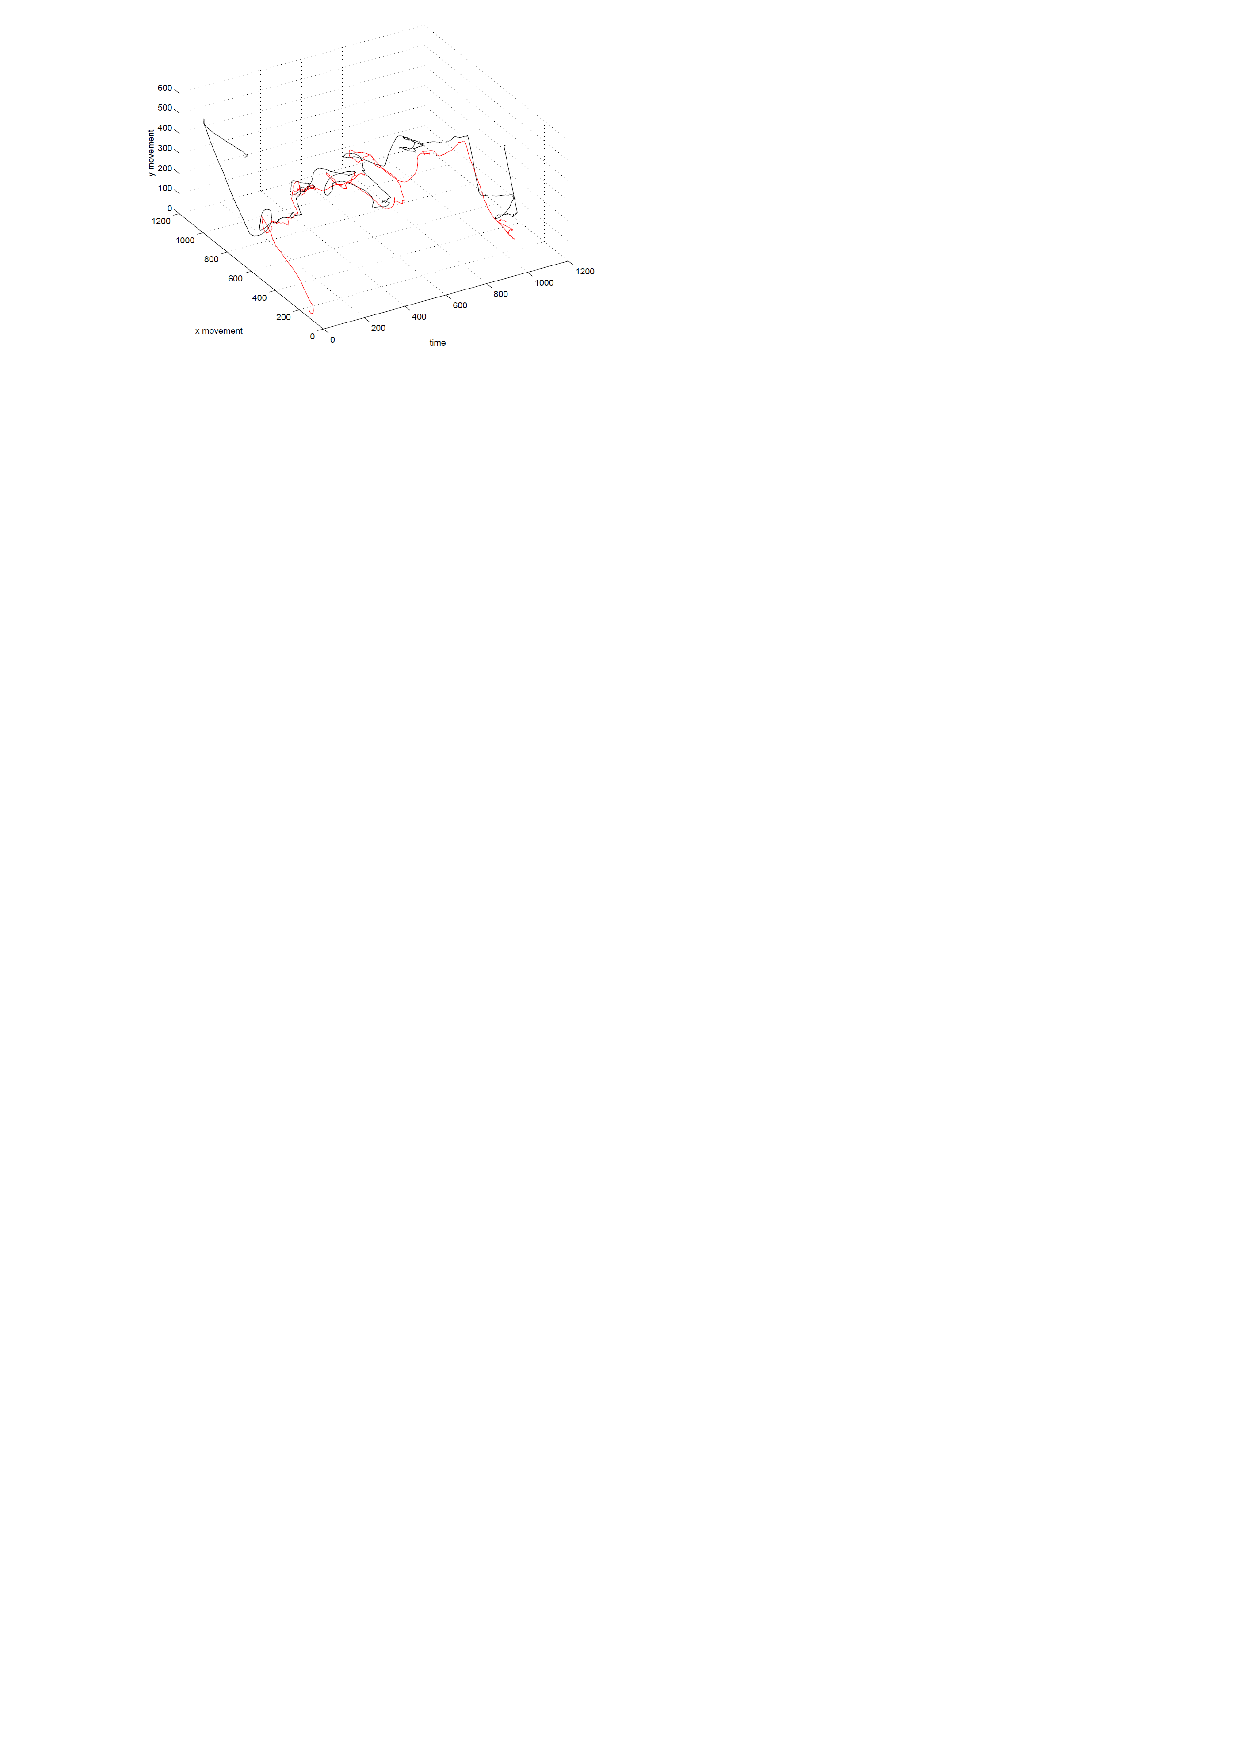
\includegraphics[scale=1]{Gambar/2d_trj}
\caption[Example of 2D trajectories with time component, from \cite{Vlachos:2002}]{Example of 2D trajectories with time component, from \cite{Vlachos:2002}} 
\label{fig:2d_trj}
\end{figure}

The trajectory of a moving object is typically modeled as a sequence of consecutive locations in a multi-dimensional (generally two or three dimensional) Euclidean space \cite{Vlachos:2002}.
Figure~\ref{fig:2d_trj} shows an example of two trajectories from two objects which are moving in a 2D plane.
With their temporal component, we can see that these trajectories are represented as polylines in a 3D space.

Nowadays, with the rapid development of technologies in mobile computing and wireless communication, many devices with location acquisition capabilities make it possible to obtain huge volumes of trajectory data from various moving objects.
Furthermore, analysis of trajectory data is an important task for many applications that contain processing and managing moving objects, such as animal movements \cite{Calenge:2009,Nams:2004,Herb:2010,Brillinger:2001}, traffic and transport analysis \cite{Yunyao:1998}, defense and surveillance areas \cite{Ng:2001}, oceanographic observations\footnote{W.S. Kessler, ``Argo work in the coral sea.''http://faculty.washington.edu/kessler/noumea/gliders/\\argo\_coral\_sea.html, March 2010.}, weather and natural phenomena \cite{Hubert:1957}, people behavior \cite{Fuentes:2001} and sports \cite{Brillinger:2007,Iwase:2002}.

Previous work on trajectory data analysis shows that there are several ways to analyze sets of trajectories.
For example, similarity between trajectories can be determined \cite{VlachosGunopoulos:2002,Lin:2005,Kreveld:2007}.
Trajectories can also be clustered into groups with similar characteristics \cite{Gaffney:1999,Lee:2007,Nanni:2006,Buchin:2009}.
Other examples are common data mining tasks such as classification \cite{Lee:2008,Garcia:2006} and outlier detection \cite{LeeHan:2008}.
Furthermore, interesting movement patterns such as flocking can also be computed from a set of trajectories \cite{Gudmundsson:2006,Buchin:2008,Gudmundsson:2007,Laube:2006}.

Even though analysis and research on trajectories has expanded in recent years, several basic concepts still need to be studied further.
Some of them are the median and the mean trajectory for a collection/set of trajectories.
The median and the mean trajectory share some common properties: they should be similar to other trajectories in the set and all parts of them should be located roughly in the middle of the set.
However, there are several important differences between them:
Firstly, the median trajectory must use only parts of trajectories in the set. 
It uses only parts of one trajectory or combines parts from many different trajectories.
This property might be a disadvantage for the median because some parts of it can be located not in the middle of the set, but in several situations this might be useful.

Figure~\ref{fig:mean_dis} shows a set of four trajectories which avoid the light-blue obstacle.
The possible mean trajectory (the black trajectory in the right-hand side of the figure) will pass through the obstacle because the mean must lie in the middle of all trajectories in the set.
In this case, it is clear that the mean trajectory is not suitable for a path of a moving object.

The median trajectory (black trajectory in the left-hand side of the figure) gives a more suitable path because it always uses parts of other trajectories.
In parts near the obstacle, the median is not really in the middle of other trajectories.

\begin{figure}
\centering
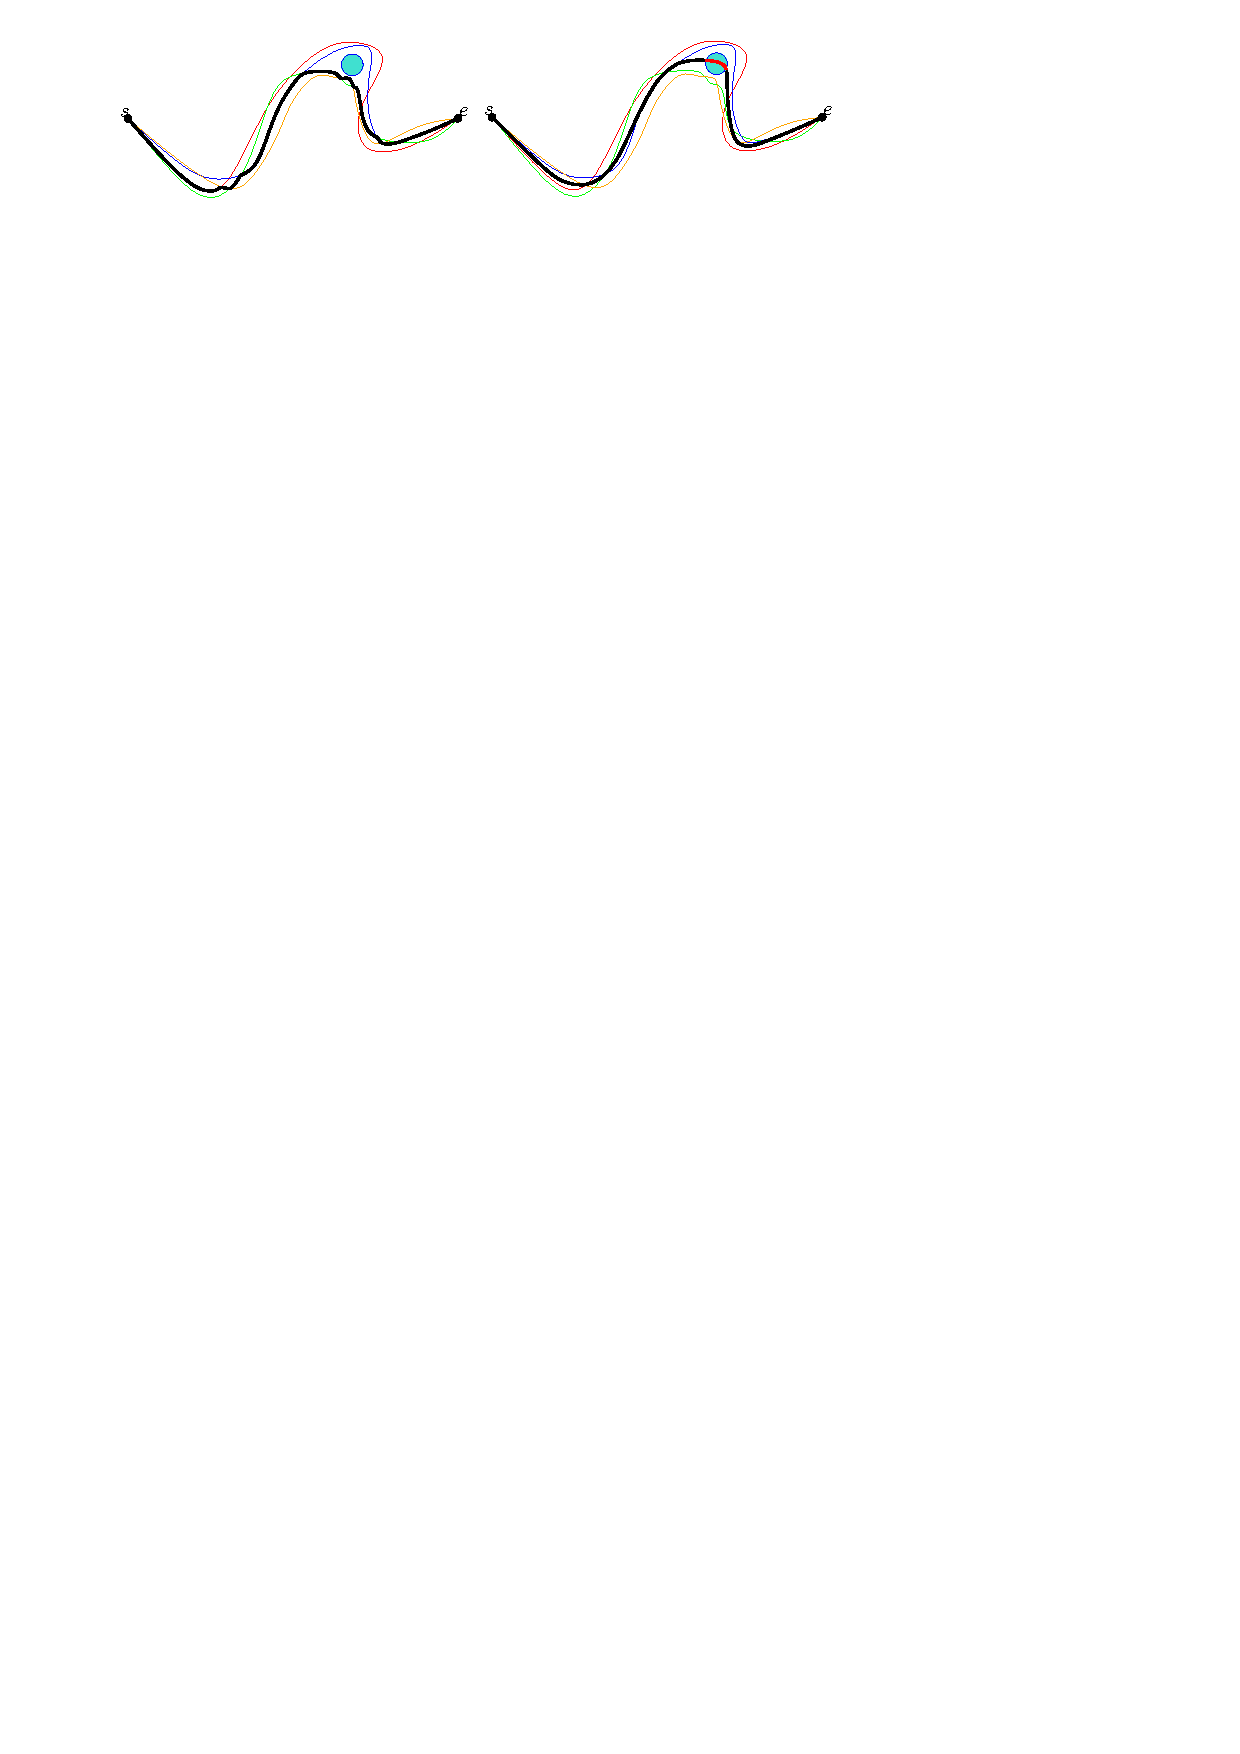
\includegraphics[scale=1]{Gambar/mean_dis}
\caption[Example of the median (left) and the mean (right) trajectory \cite{Lionov:2009}]{Example of the median (left) and the mean (right) trajectory \cite{Lionov:2009}} 
\label{fig:mean_dis}
\end{figure}

Secondly, the median trajectory is more robust against outliers than the mean trajectory.
Figure~\ref{fig:robust_med} shows this situation: we add one trajectory (with purple color) which can be categorized as an outlier compared to other trajectories. 
While the median trajectory only needs to be modified a little bit, the mean trajectory has to be changed a lot (comparing to the mean trajectory in Figure~\ref{fig:mean_dis}), to keep it in the middle of other trajectories.

\begin{figure}
\centering
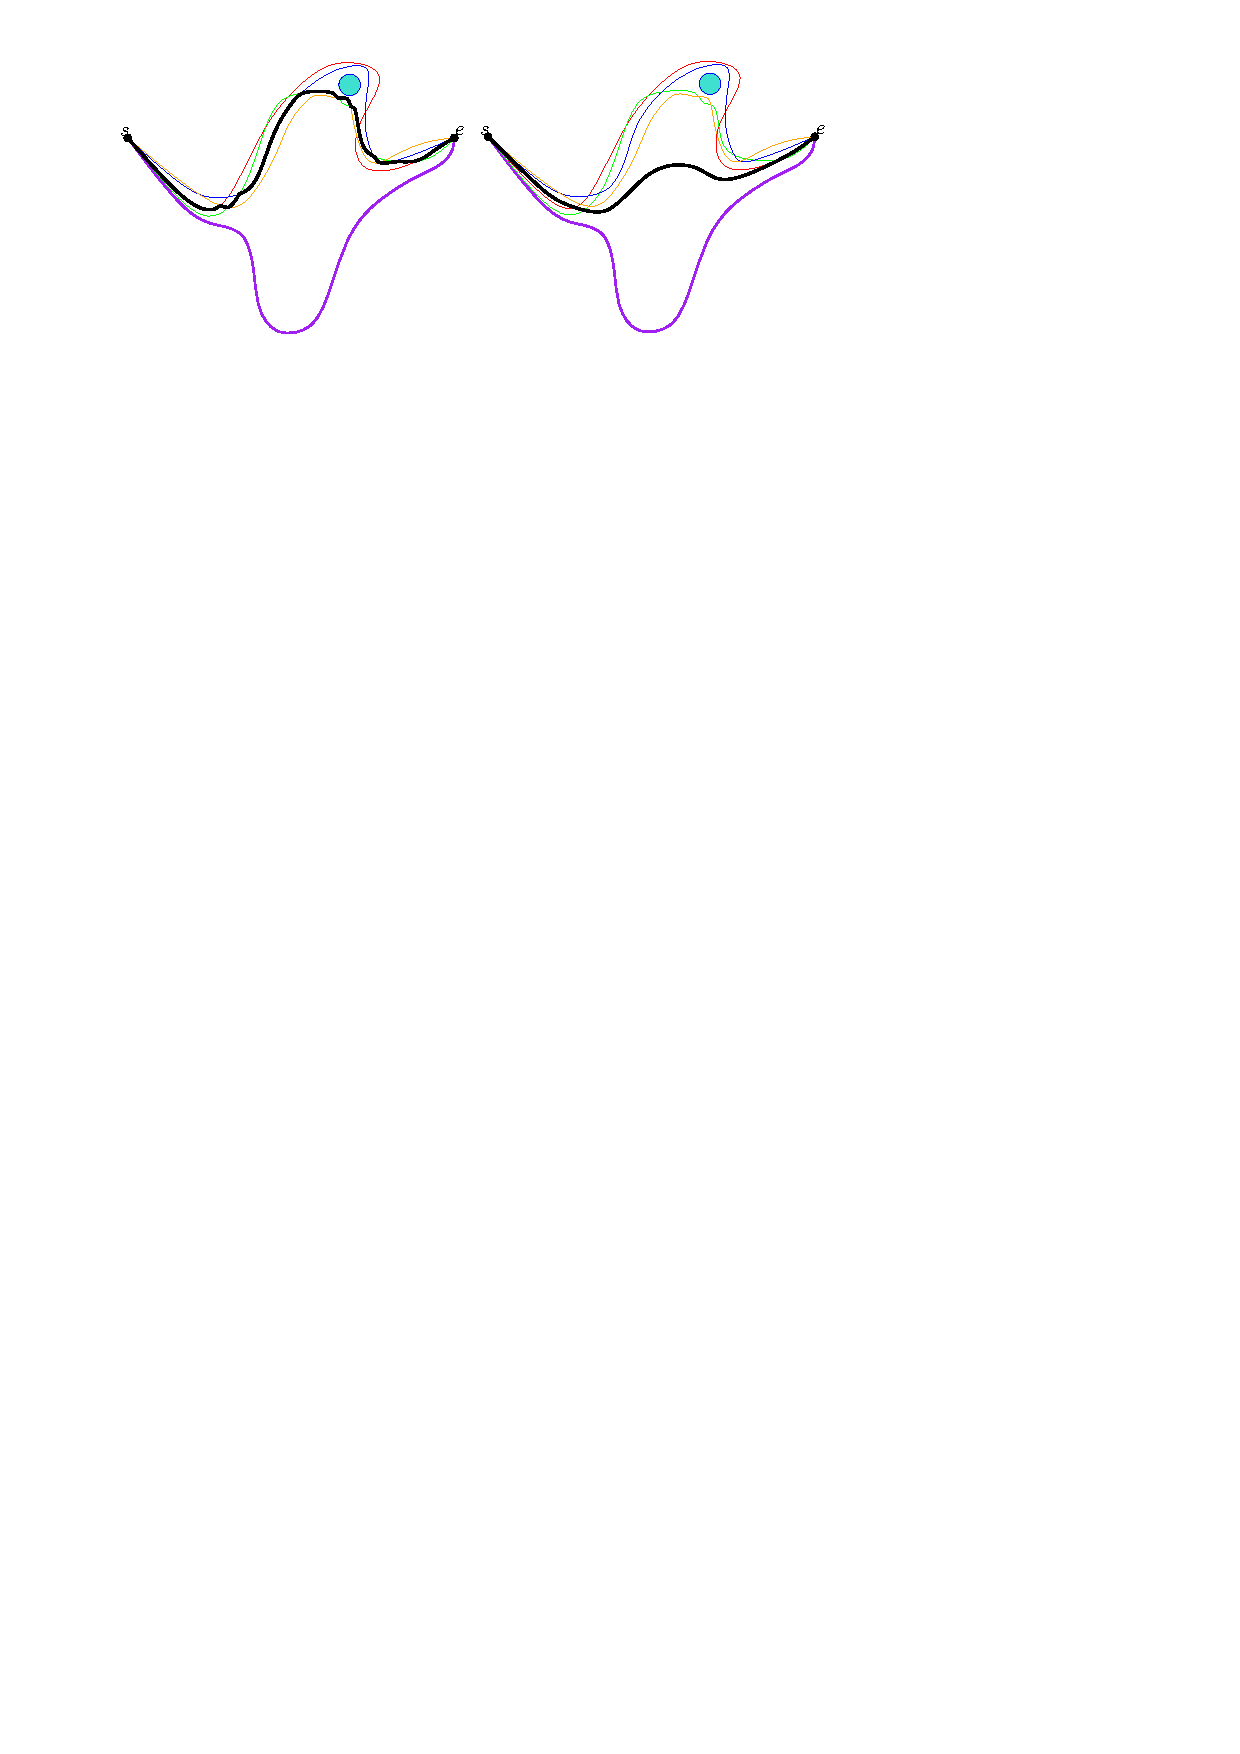
\includegraphics[scale=1]{Gambar/robust_med}
\caption[Robustness of the median trajectory]{Robustness of the median trajectory} 
\label{fig:robust_med}
\end{figure}

In this thesis, we will not cover the mean trajectory and only discuss the median trajectory and algorithms to compute it.
We also ignore the temporal component of the trajectory because it is not clear yet how to take it into account when computing the median trajectory. 
However, some research on motion and kinetic data structures contains a temporal component and are related to the median/mean trajectory \cite{Agarwal:2003,Agarwal:1997}. 

For other types of data, a median has a clear definition.
The median from a population (or a sample) of integer numbers is the number that separates the population into two halves, where at most half of the population have a smaller value and the other half of the population have a larger value than the median. 

For geometric data types, the concept of median also exist.
A \textit{center point} of a set $P$ of $n$ points in the plane is a point such that any closed half-plane whose bounding line contains the center point, contains at least $n/3$ points of $P$ \cite{Amenta:2000}.
If we force the center point to be one of the points from $P$, then we obtain a 2-dimensional version of the median, although the ``quality'' of this median can be bad.

The median trajectory does not have any formal definition yet.
Based on several properties that we mention earlier, such as its similarity with other trajectories and lying approximately in the middle of the set, we can determine a possible median, which can useful in several ways:

\subsection{Determine the most typical trajectory}
The property of the median trajectory makes it suitable to analyze the movement behavior or movement pattern from a group of same objects because the median somehow represents the whole trajectories in the set/collection.
The median trajectory properties, such as the length, the direction or the average speed (if we include the temporal component), could give valuable information.

Example applications include the detection of outliers, which can be done by analyzing the length and the similarity of the shape of the median with other trajectories.
Analyzing the average speed together with the shape of the median trajectory might be useful to understand the behavior and the movement pattern of people walking around in an area which has several interesting places to be visited (e.g., a zoo or an amusement park). 

\subsection{Better visualization for a set of trajectories}
Visualization of the median trajectory, together with its set of trajectories, might give the viewer a better interpretation and information about the set of trajectories.

\begin{figure}
\centering
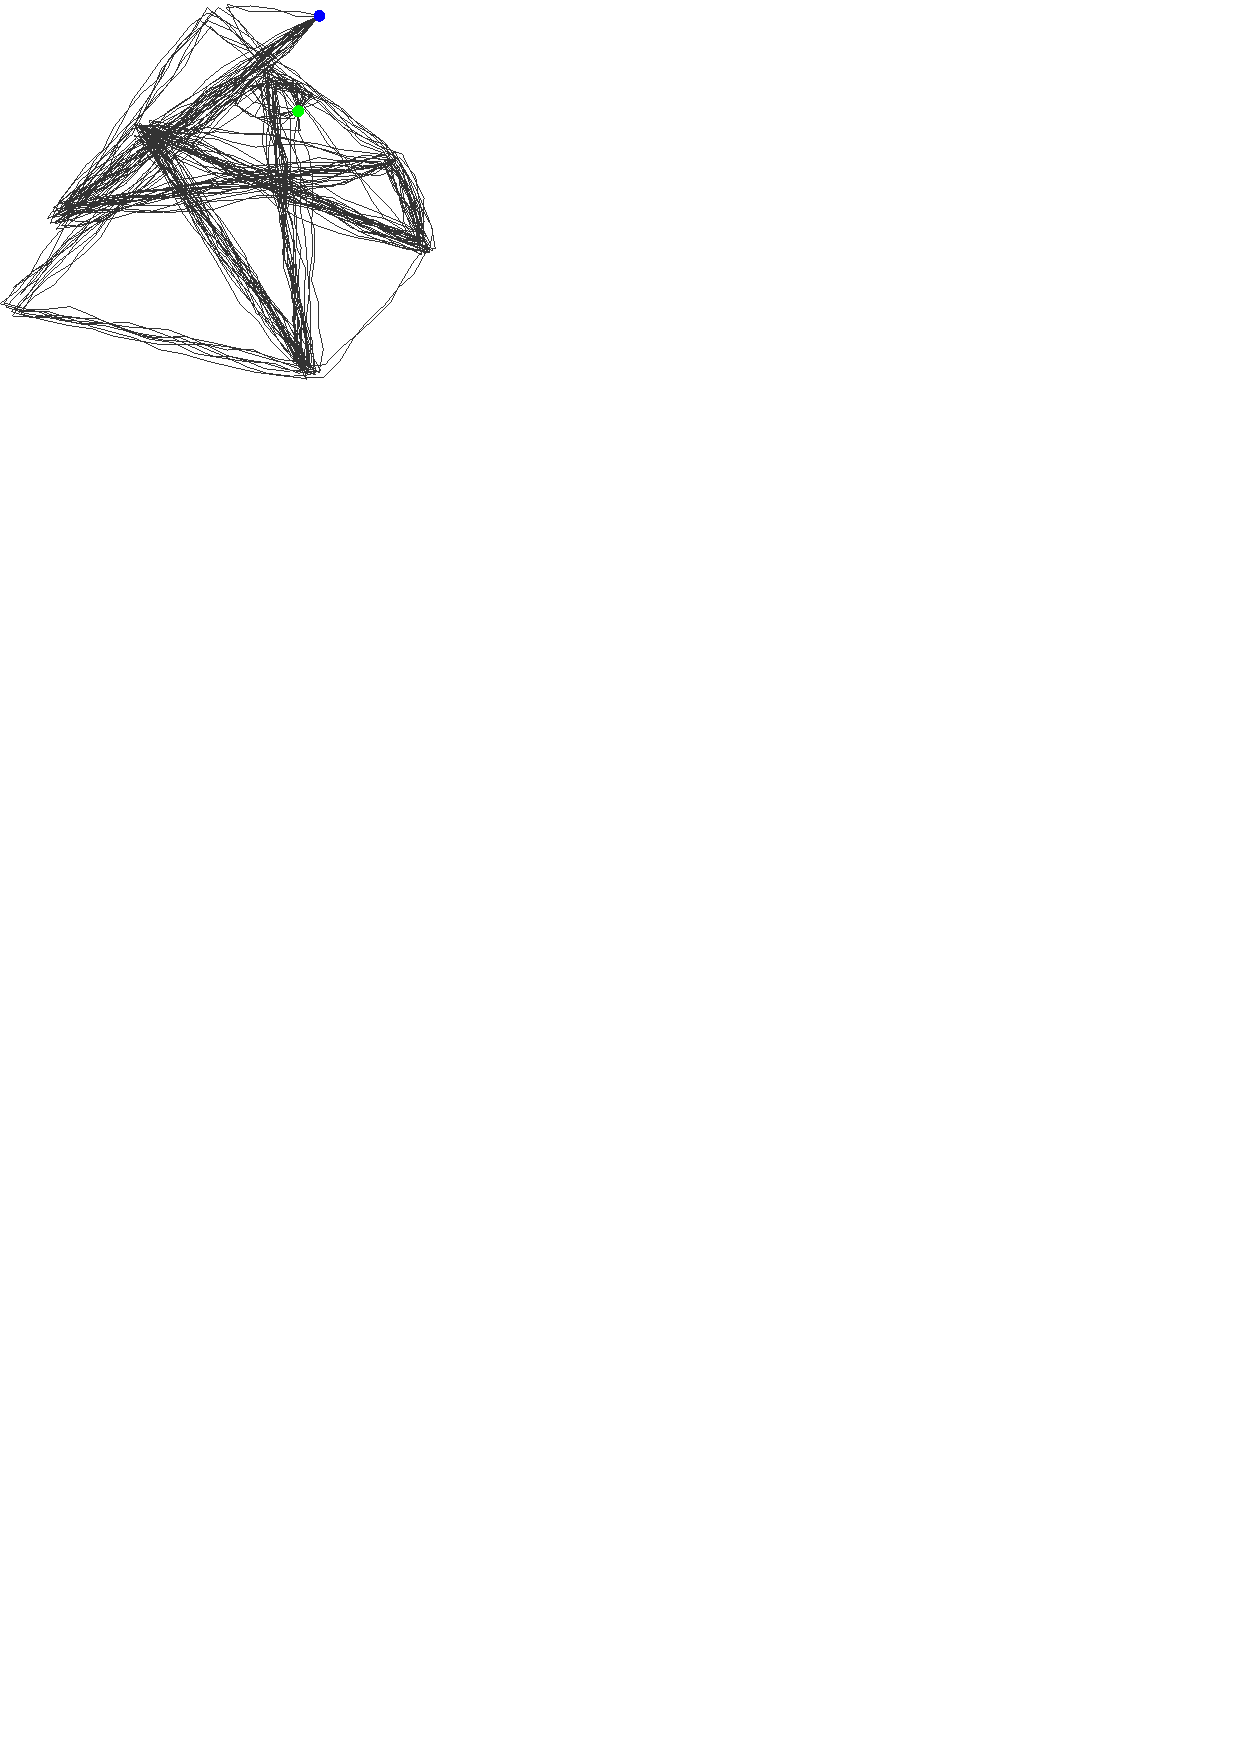
\includegraphics[scale=1]{Gambar/all30_visual}
\caption[The set of 30 trajectories, starting at the blue point \& ending at the green point]{The set of 30 trajectories,starting at the blue point \& ending at the green point} 
\label{fig:all30_visual}
\end{figure}

\begin{figure}
\centering
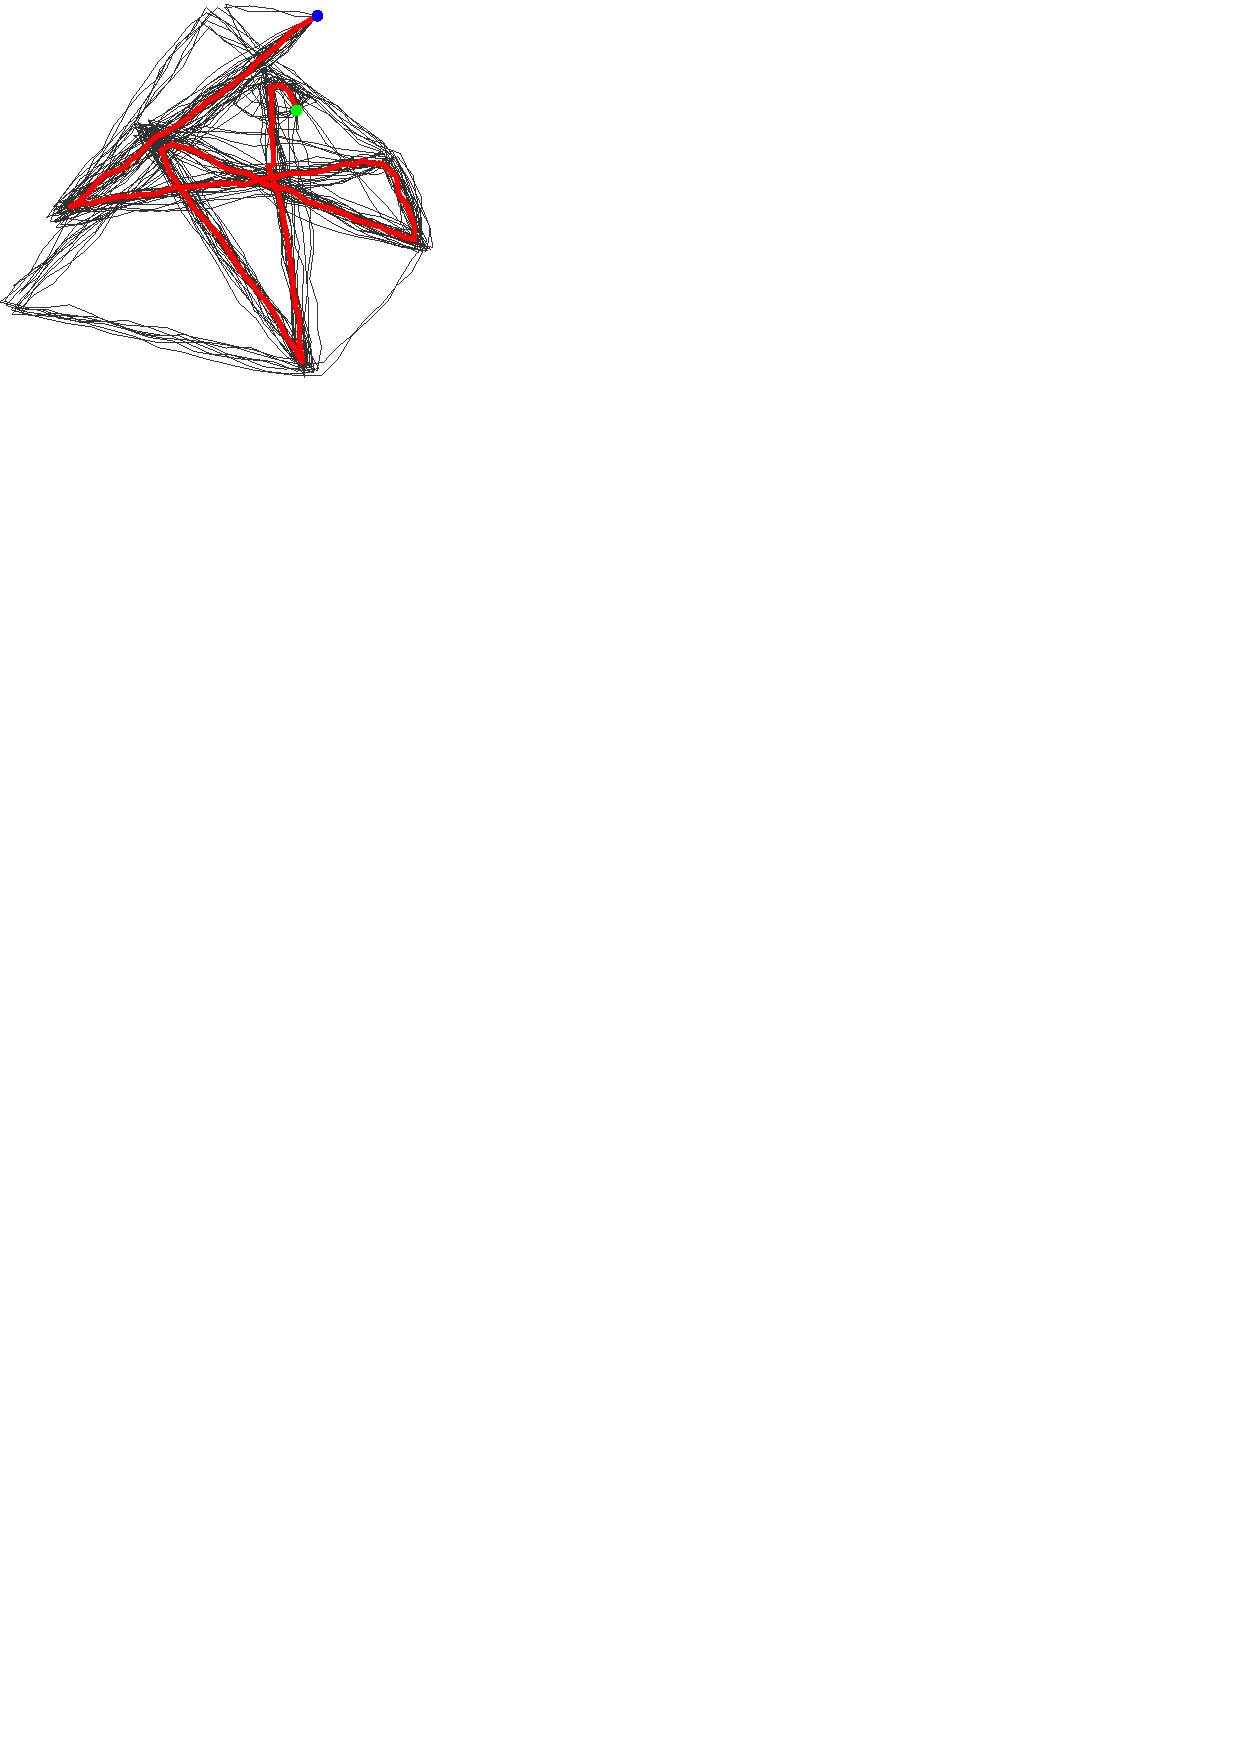
\includegraphics[scale=1]{Gambar/med_visual}
\caption[A set of 30 trajectories with its possible median trajectory]{A set of 30 trajectories with its possible median trajectory} 
\label{fig:med_visual}
\end{figure}

We give an example in Figure~\ref{fig:all30_visual}, where a set has 30 trajectories, which is paths of 30 objects moving from the blue point to the green point.
From this figure, we can hardly tell anything about the general behavior or the direction of these trajectories. 
However, we know that several trajectories are different than others and probably can predict what the majority does, but it is still difficult to visualize what the majority of these trajectories does.

In the following figure (Figure~\ref{fig:med_visual}), we present a possible median trajectory as the red and thick trajectory.
From this visualization, it is clear what the majority of trajectories does.
Moreover, we can identify what parts of some trajectories are completely different from others. 

The visualization of the median trajectory could be useful in some real-life applications:
The median trajectory from trajectories of visitors in a national park can be used to see the most common path taken by visitors, which is probably the path that is preferred by future visitors.
This information might be useful if we want to create a map that can help those visitors by providing valuable information about a path and direction on that national park in the map, so that he/she can decide which path that he/she will take. 
% Other example is to use the median trajectory for video surveillance. 
% where median trajectory shows the most common path that the visitor take, and identify if there are any unusual trajectory

\subsection{\texorpdfstring{$k$}{k}-medoid clustering}
Another application that could use the median trajectory is the $k$-medoid algorithm, which is used in cluster analysis.
The $k$-medoid clustering algorithm is related to the $k$-means algorithm, a method to partition/group a set of objects into $k$ different clusters containing similar objects.

In general, each cluster in both algorithms has one object act as a \textit{central object} and other members of the cluster should be similar or having a small distance to this object.
The similarity or the distance between objects can be measured using different distance functions (e.g. Euclidean distance, Minkowski distance, etc), depending on the type of objects and the purpose of the clustering.

The main difference between the two algorithms is on the selection of the central object for each cluster. 
While the $k$-means simply uses the mean of objects, the $k$-medoid must use the medoid (an object which has the smallest average of dissimilarity/distance to all other objects in the set, but it must be a member of the set). 
This implies that $k$-means could create a new object to be the central object whereas the $k$-medoid must use one of the objects from the set.
Thus, the $k$-medoid algorithm is more suitable for spatial clustering purposes and less sensitive against noise and outliers.  

Partitioning Around Medoids (PAM) ~\cite{Kaufman:2005} is a basic $k$-medoid clustering algorithm.
It works as follow:
\begin{enumerate}
\item
Define a value $k$ and choose $k$ objects as a set of medoids.
\item
Assign every object to its closest/similar medoid and after that, compute the cost for the whole configuration.  
\item
Find another configuration by selecting a pair of medoid and non-medoid objects which have the smallest distance cost and swapping them temporarily.
Then, we assign all other objects to this temporary set of medoids and obtain a new configuration.
\item
If the new configuration has smaller cost than the last configuration, then we change the set of medoids and return to step 3
\item
Otherwise, stop and we find the set of medoids with their non-overlapping set of clusters.
\end{enumerate}

In case we want to cluster a set of trajectories, we can use the median trajectory as a medoid in this algorithm.
However, some changes probably should be made.
For example, finding another configuration is not done by simply swapping the median with other trajectory, instead we can choose to swap part of them (with the requirement that both trajectories intersect one another).

\section{Basic Idea of the Research}
\label{sec:basic_idea}

Consider a set $T$ of $m$ trajectories.
We want to to compute the median trajectory of $T$.
In this set, all trajectories have the same start and end points.
The median trajectory of $T$ must be built using parts of trajectories in $T$ and somehow must follow what other trajectories in $T$ do, while staying in the ``middle'' of other trajectories.

\subsection{The Simple Switching Method }
\label{sec:switch}

A simple idea to obtain a median trajectory from $T$ is to start from the ``middle'' trajectory, which is the $(m+1)/2$-level of arrangement formed by all trajectories in $T$ (we assume $m$ is odd).
At every intersection point, the median trajectory will switch to another trajectory and keep $(m+1)/2$ trajectories above and below the median \cite{Buchin:2010}.

\begin{figure}
\centering
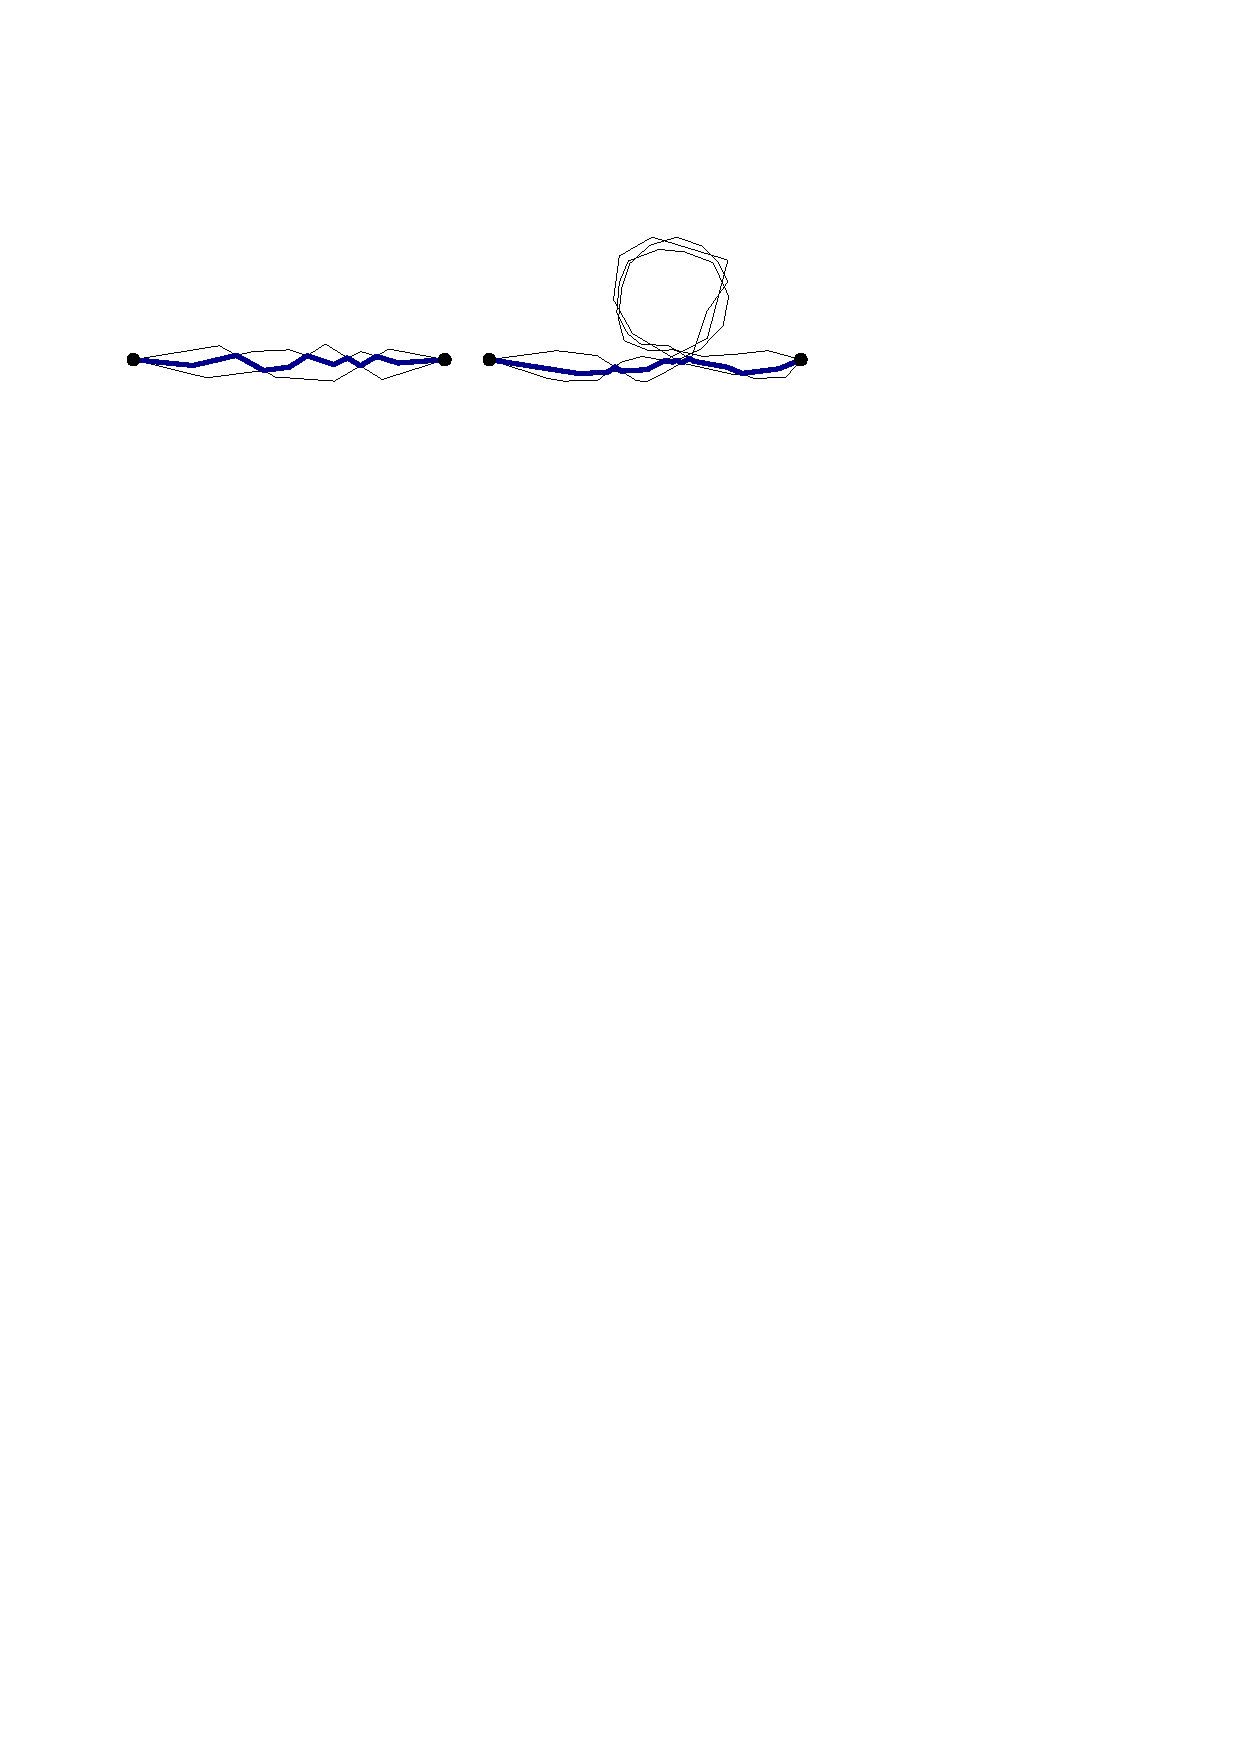
\includegraphics[scale=1]{Gambar/switch_fail0}
\caption[Illustration of the simple idea using switching]{Illustration of the simple idea using switching} 
\label{fig:switch_fail0}
\end{figure}

\begin{figure}
\centering
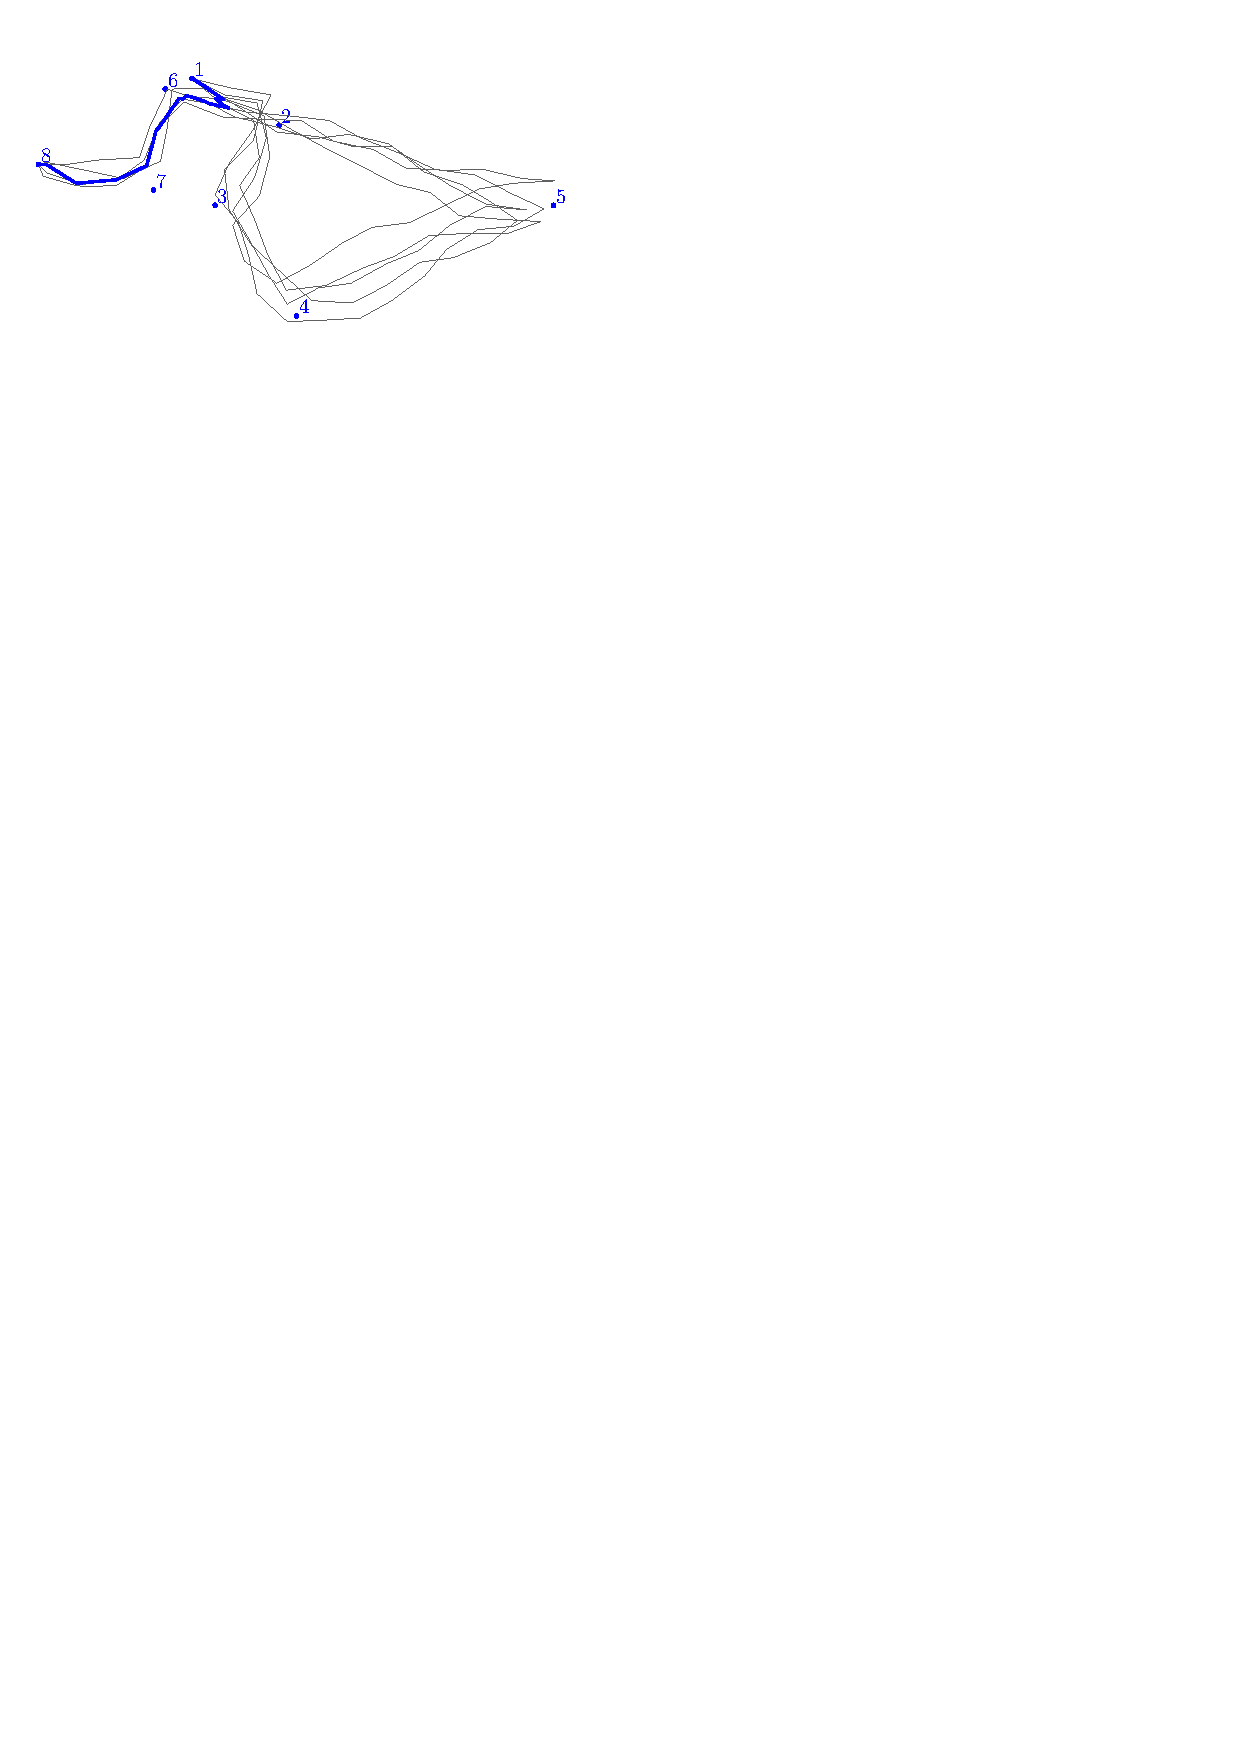
\includegraphics[scale=1]{Gambar/switch_fail1}
\caption[The median trajectory make a shortcut path \cite{Lionov:2009}]{The median trajectory makes a shortcut \cite{Lionov:2009}} 
\label{fig:switch_fail1}
\end{figure} 

Figure~\ref{fig:switch_fail0} shows the result (the median trajectory is the thick-blue trajectory) of this approach for two different types of set of trajectories, one of them contains trajectories with self intersection.
From the right-hand side of the figure in Figure~\ref{fig:switch_fail0}, we can see that this method cannot produce suitable median trajectory because the median does not follow the loop created by the three trajectories.

In general, this method will not give a suitable median if a set of trajectories contains self-intersecting trajectories.
More examples from \cite{Lionov:2009} show several ``incorrect'' median trajectories obtained by using this simple switching method.
The blue median trajectory in Figure~\ref{fig:switch_fail1} makes a shortcut path to the end point.

\begin{figure}
\centering
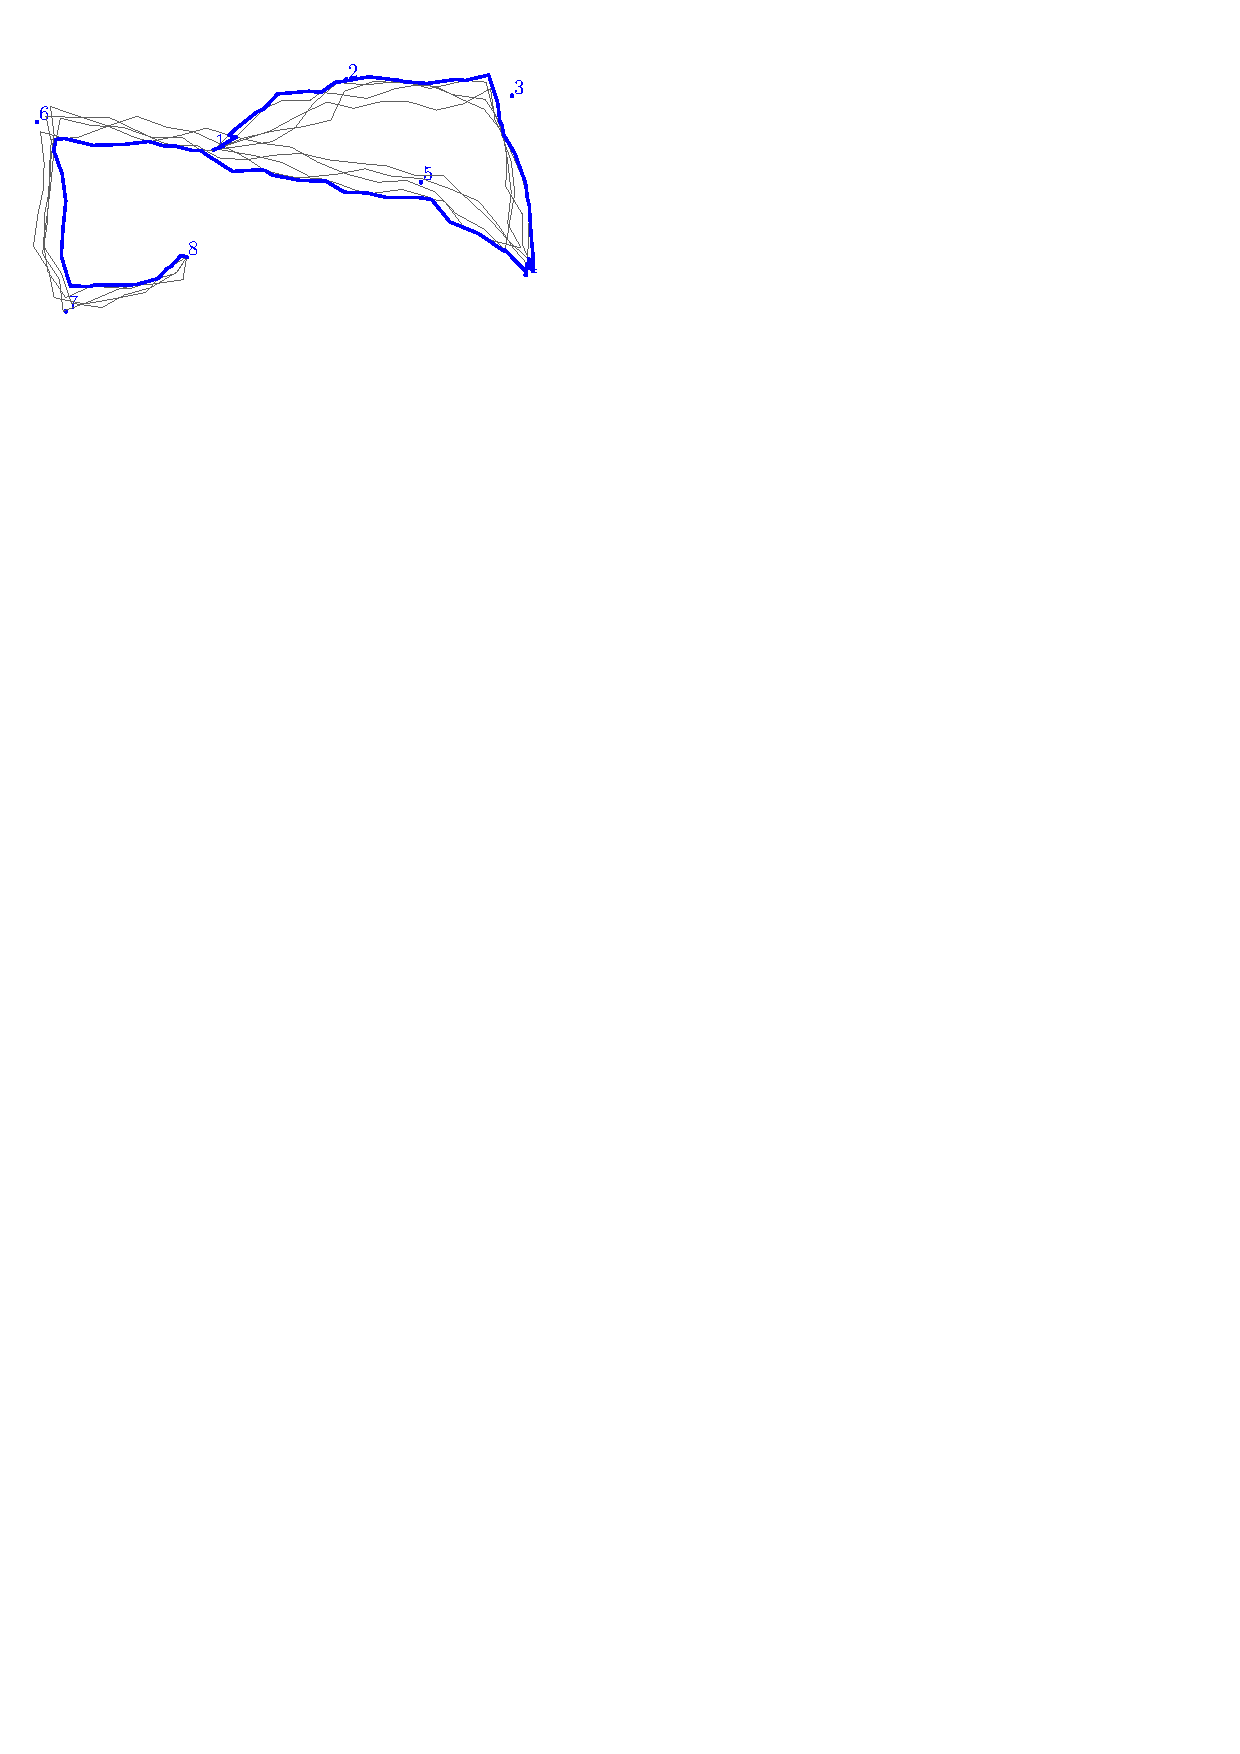
\includegraphics[scale=1]{Gambar/switch_fail2}
\caption[The median trajectory does not stay in the middle \cite{Lionov:2009}]{The median trajectory does not stay in the middle \cite{Lionov:2009}} 
\label{fig:switch_fail2}
\end{figure} 

The median trajectory in Figure~\ref{fig:switch_fail2} does not stay in the "middle" of other trajectories.
Finally, in Figure~\ref{fig:switch_fail3}, the median trajectory does not follow the sequence of regions as the other trajectories. 
The correct sequence of regions is $1-2-3-4-5-6-7-8$.

\begin{figure}
\centering
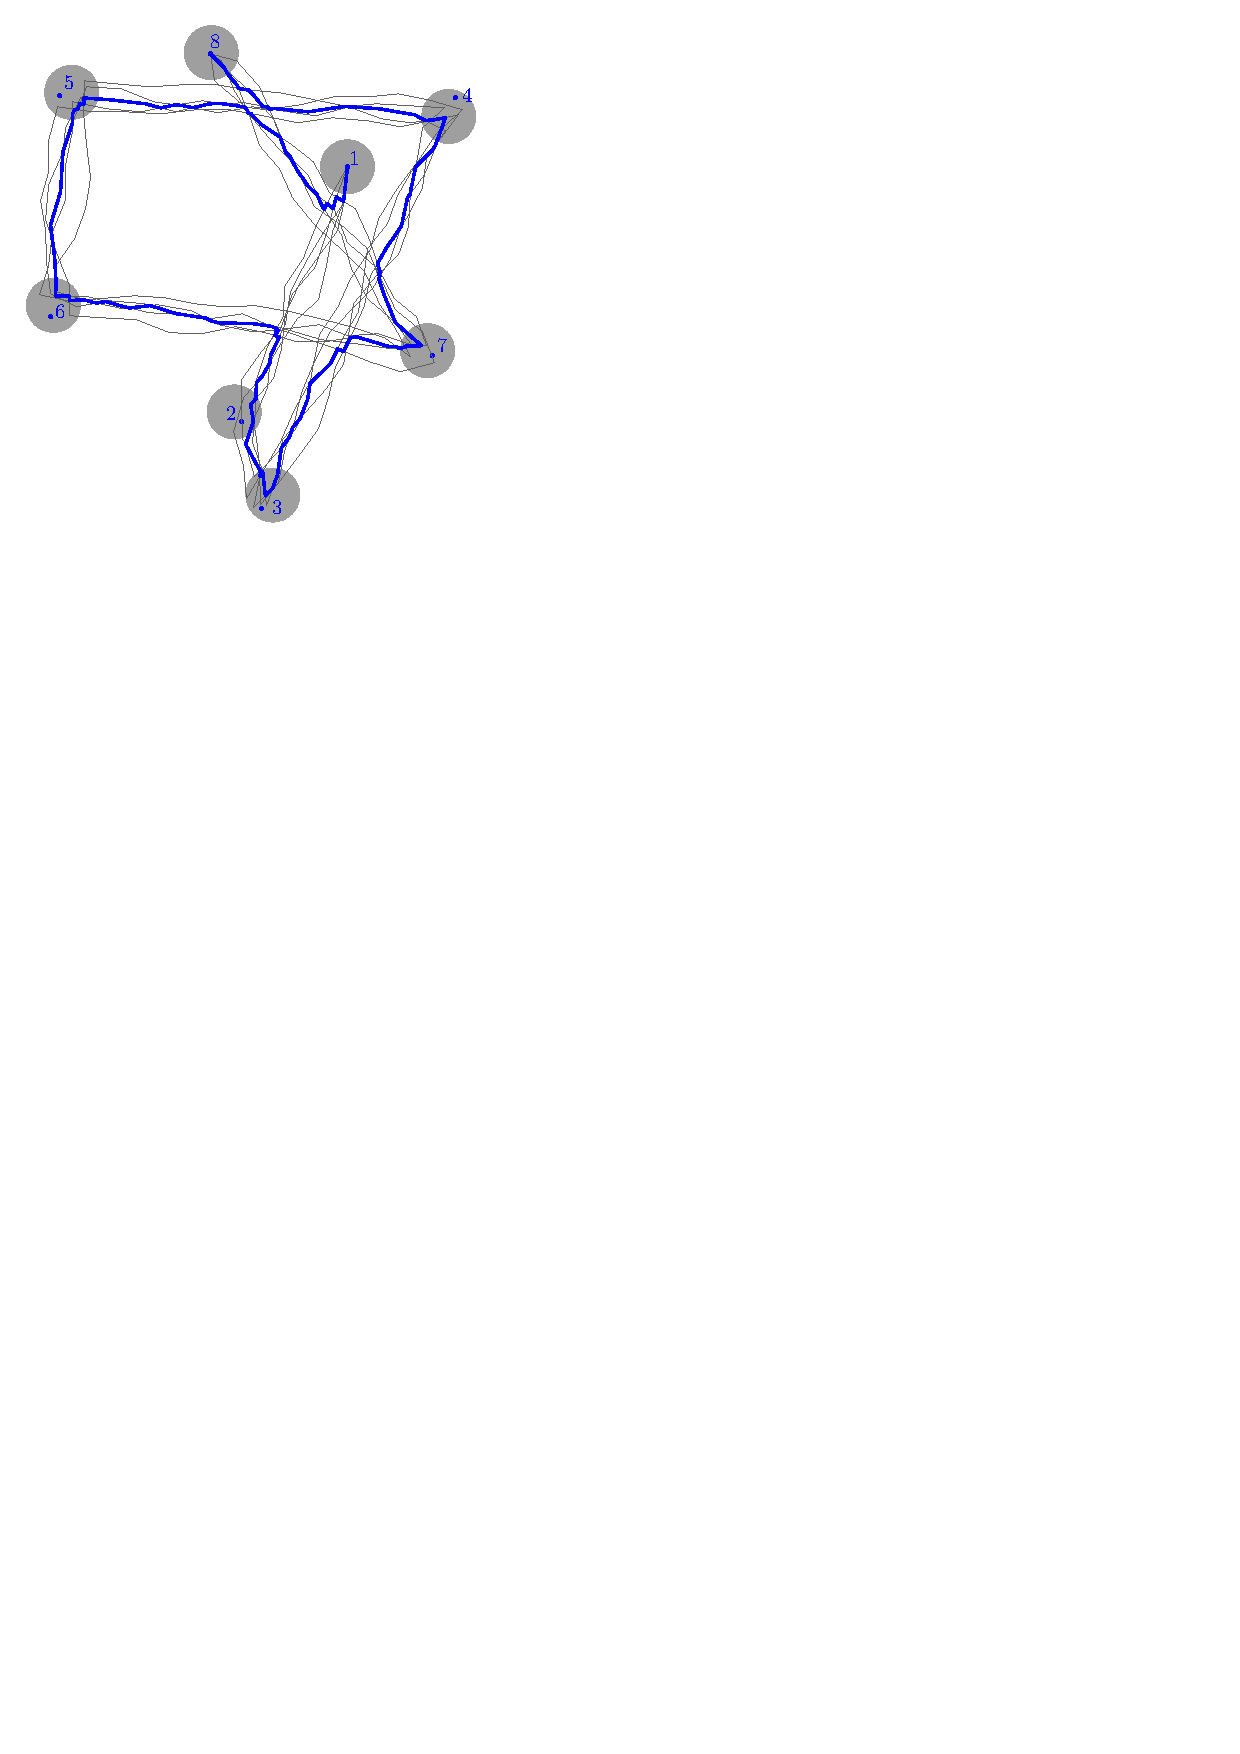
\includegraphics[scale=1]{Gambar/switch_fail3}
\caption[The median trajectory follows incorrect direction \cite{Lionov:2009}]{The median trajectory does not follow the correct sequence of regions \cite{Lionov:2009}} 
\label{fig:switch_fail3}
\end{figure} 
 
\subsection{The Algorithm Using the Concept of Homotopy}
\label{sec:homotopy}

Another algorithm to compute the median trajectory uses the concept of homotopy (along with the modified simple switching method) \cite{Buchin:2010}.
This algorithm works by placing cross in a relatively large face bounded by segments from a set of trajectories.
Figure~\ref{fig:homotopy} shows an example where cross is placed in the relatively large bounded face and two crosses are placed in the outer face.

\begin{figure}
\centering
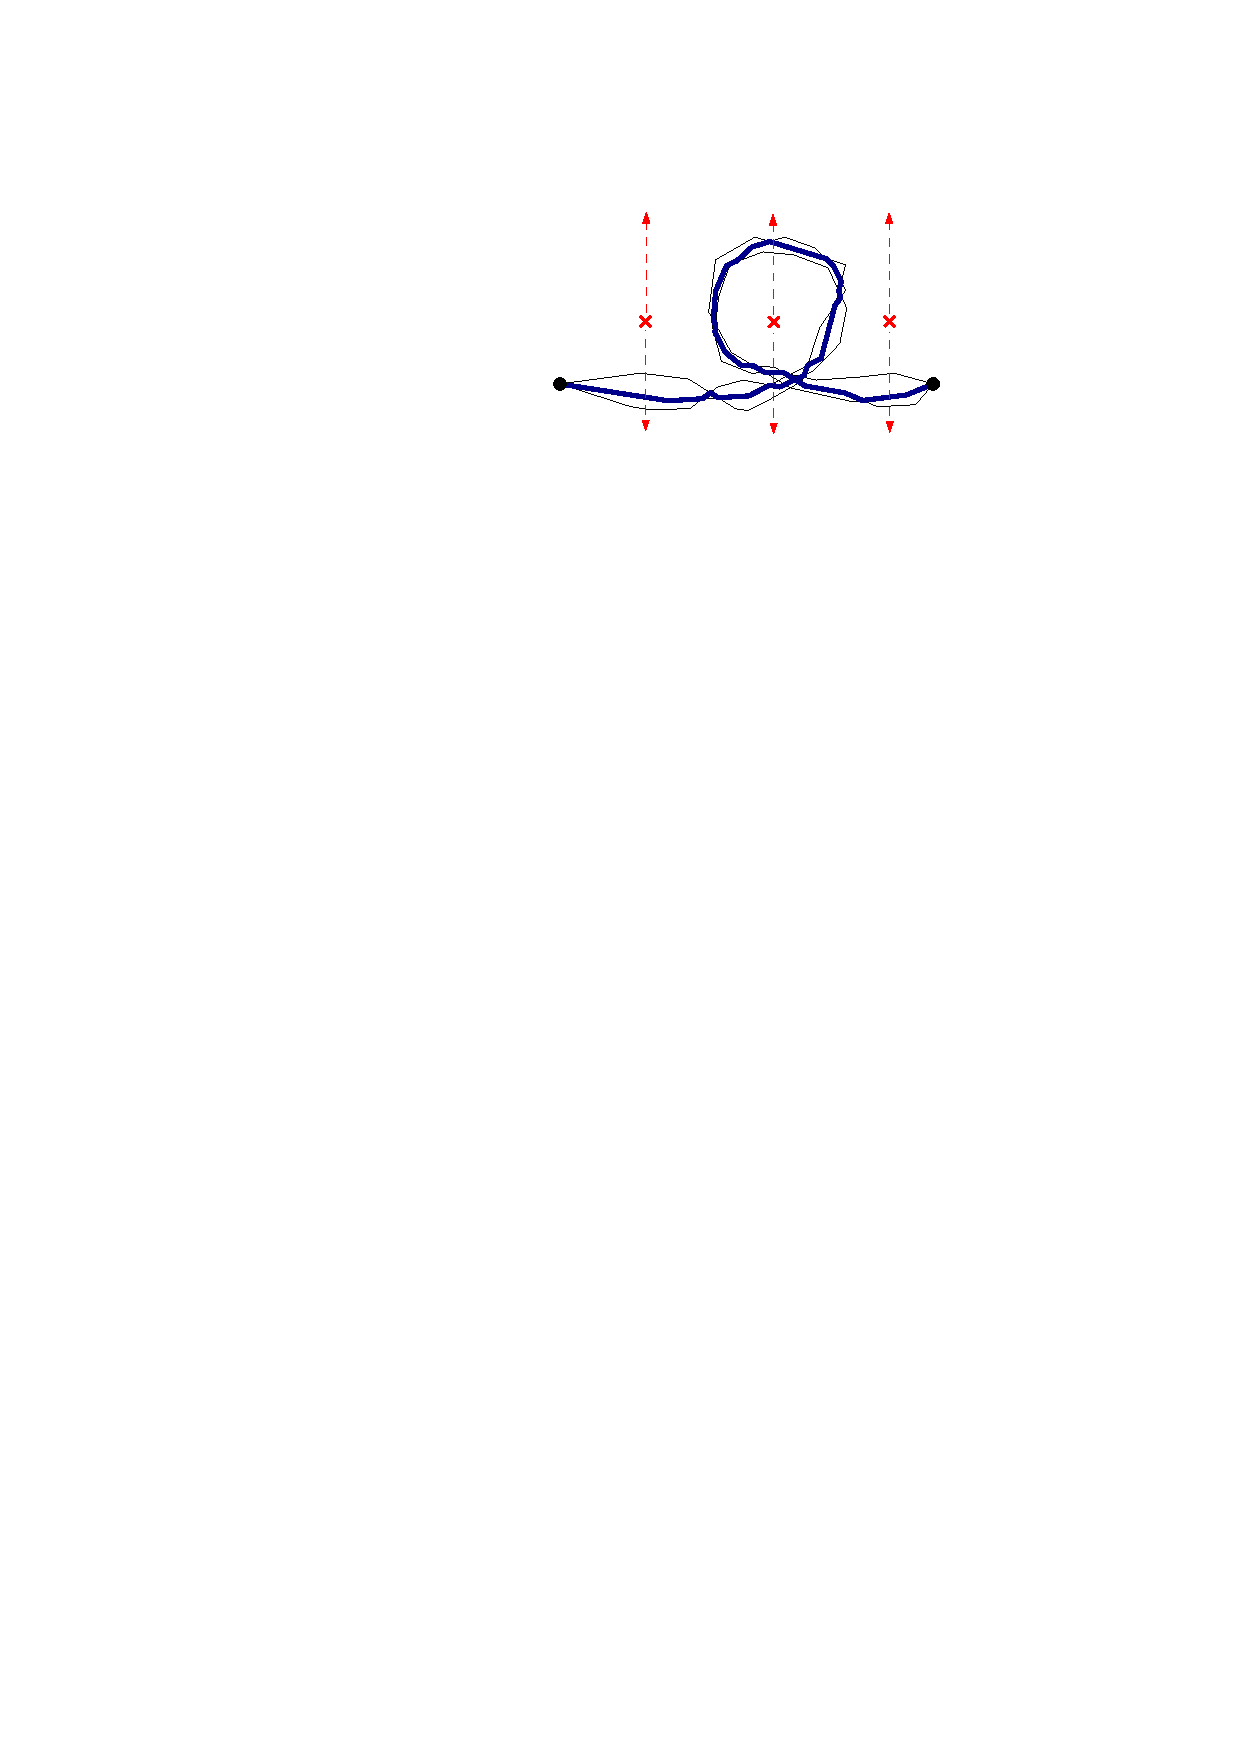
\includegraphics[scale=1]{Gambar/homotopy}
\caption[Illustration of the algorithm using homotopy concept]{Illustration of the algorithm using homotopy concept} 
\label{fig:homotopy}
\end{figure}

Based on the location of these crosses, each trajectory in $T$ will be assigned a \textit{signature}.
Figure~\ref{fig:base_sign} shows three trajectories and two crosses \textit{a} and \textit{b}. 
From these two crosses, four half-lines are created: \textit{$a^{+}$} and \textit{$a^{-}$} are half-lines above and below \textit{a}, while \textit{$b^{+}$} and \textit{$b^{-}$} are half-lines above and below \textit{b}, respectively. 

For all trajectories in $T$, we give them a signature based on how they intersect with the half-line(s) from the crosses. 
Note that each trajectory might have a different signature, because it depends on the position of the trajectory with respect to all crosses in the plane.
In Figure~\ref{fig:base_sign}, the blue trajectory intersect with \textit{$a^{-}$} and \textit{$b^{+}$}, thus its signature will be \textit{$a^{-}b^{+}$} (the order is following the direction of the trajectory). 
In the same way, the signature of the red trajectory will be the same as the green trajectory: \textit{$a^{-}b^{-}$}.

\begin{figure}
\centering
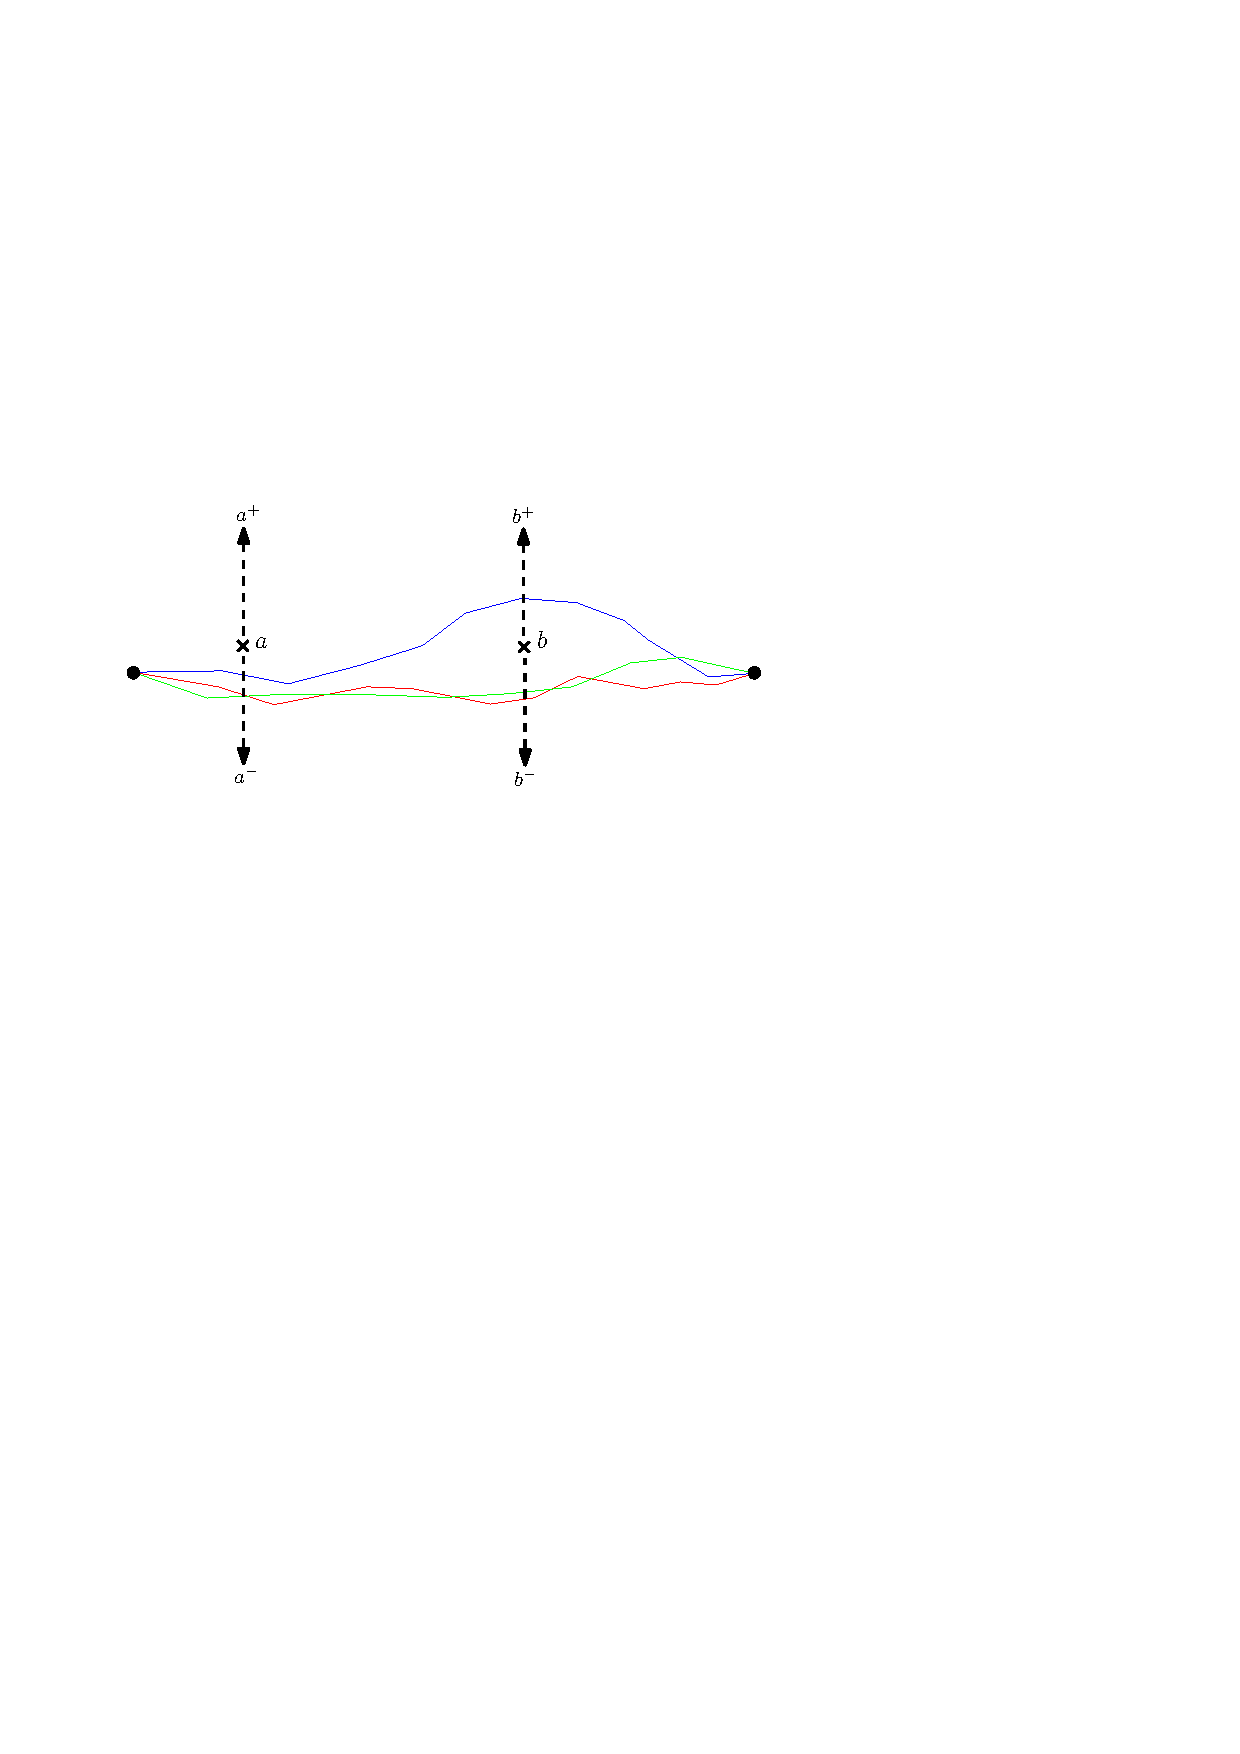
\includegraphics[scale=1]{Gambar/base_sign}
\caption[Trajectories and crosses]{Trajectories and crosses} 
\label{fig:base_sign}
\end{figure}

% The next step of the algorithm is to create the subset $T'$ of $T$.
% All trajectories in $T'$ must be homotopic to each other and also the set with the most number of trajectories from $T$.

Two different trajectories are homotopic if one trajectory can be deformed continuously into the other one without passing through any crosses, while the start and end point are not moved.
Naturally, two trajectories are homotopically equivalent if their signatures are exactly the same. 
However, two homotopic trajectories do not always have the same signatures.
We shown an example in Figure~\ref{fig:diff_sign} where the blue and the black trajectory are homotopic, but their signatures are different.

To determine whether two trajectories with different signature are homotopic or not, we perform a \textit{reduce} operation.
This \textit{reduce} operation works by eliminating two exact same signs, if their position is next to each other in the signature.
In Figure~\ref{fig:diff_sign}, the signature of the blue trajectory is \textit{$a^{-}b^{+}c^{+}c^{+}b^{+}b^{-}c^{-}$}.
Notice that it has two \textit{$c^{+}$} that we can eliminate.
This will change the signature of the blue trajectory into \textit{$a^{-}b^{+}b^{+}b^{-}c^{-}$}.
Once again, we can identify that two \textit{$b^{+}$} are positioned directly to each other. 
Performing the reduce operation again, we will get the final signature of the blue trajectory: \textit{$a^{-}b^{-}c^{-}$}.
At this point, we cannot apply the reduce operation again to this signature, and we say that the signature has been \textit{maximally reduced}.
Finally,we conclude that if two trajectories have the same maximally reduced signature, then the two trajectories are homotopically equivalent.  

\begin{figure}
\centering
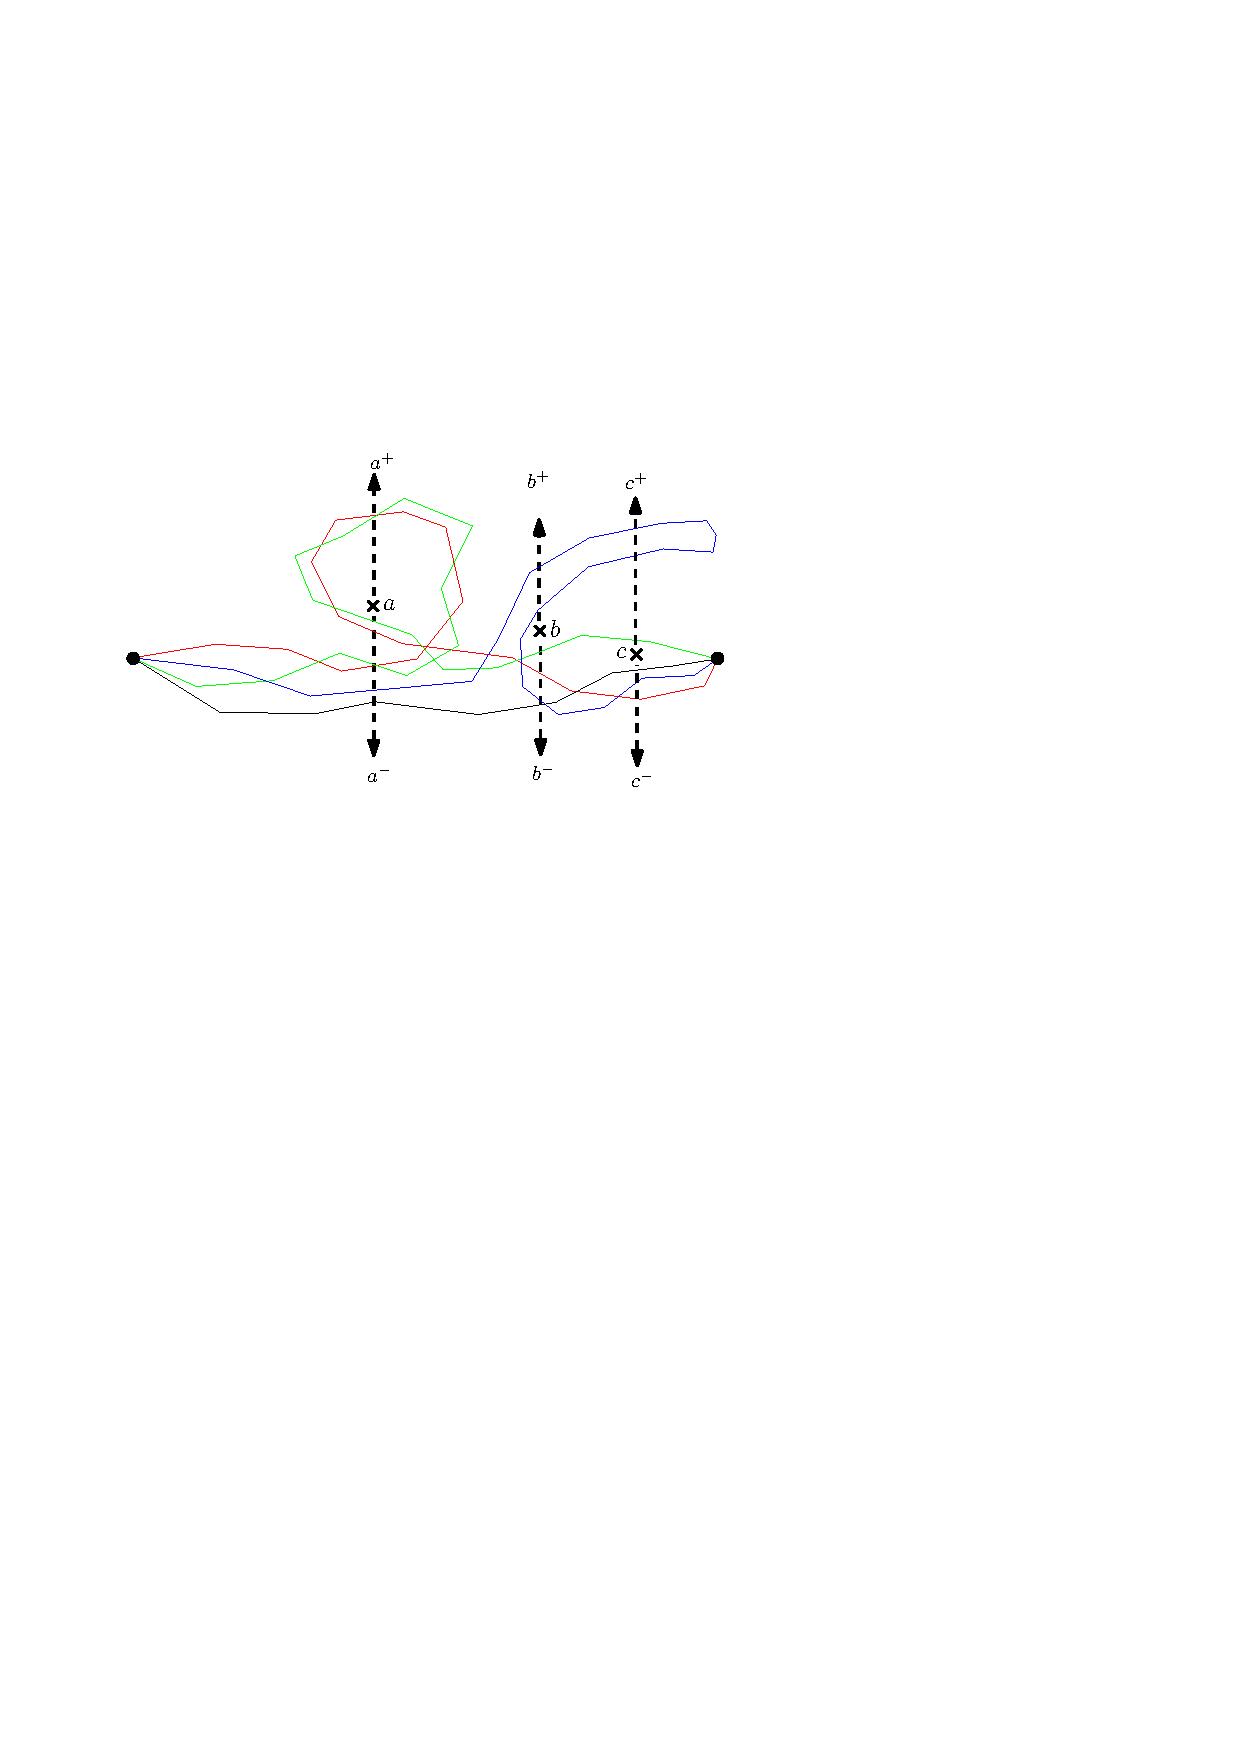
\includegraphics[scale=1]{Gambar/diff_sign}
\caption[The blue and black trajectory are homotopically equivalent \cite{Lionov:2009}]{The blue and black trajectory are homotopically equivalent \cite{Lionov:2009}} 
\label{fig:diff_sign}
\end{figure}

The next step of the algorithm is to create a subset $T'$ of $T$, and then find the median trajectory by using only parts of trajectories from $T'$.
Creating $T'$ is straightforward, we only need to compute maximally reduced signature for all trajectories and choose a subset with the largest number of trajectories which have the same signature.

To create the median trajectory from $T'$, we use the modified version of the switching method.
This method start at the first segment of the``middle'' trajectory.
We find such a segment by determine the outer face of the set of trajectories.
The first segment of the ``middle'' trajectory is the segment where there are $(n-1)/2$ first segments from other trajectories (assume $n$ is odd) between the segment and the outer face (on each side of the segment).
% The algorithm starts with the trajectory which $(n-1)/2$ trajectories in $T'$ are above and the rest are below it (assume $n$ is odd).


Then, at every intersection, the median will switch to another trajectory if the continuation along this trajectory (without ever switching again) gives the same signature with the signature of one trajectory from $T'$.
Figure~\ref{fig:homotopy_algo} shows an example of this algorithm.
After starting with the red trajectory and switching to the green trajectory at the first intersection, the next intersection is with the blue trajectory (at the small blue square) and so far, the signature for the median is \textit{$a^{+}$}. 
Although the blue trajectory is going forward, the signature after this intersection while following the blue trajectory (until the end point) is \textit{$b^{-}c^{-}$}. 

\begin{figure}
\centering
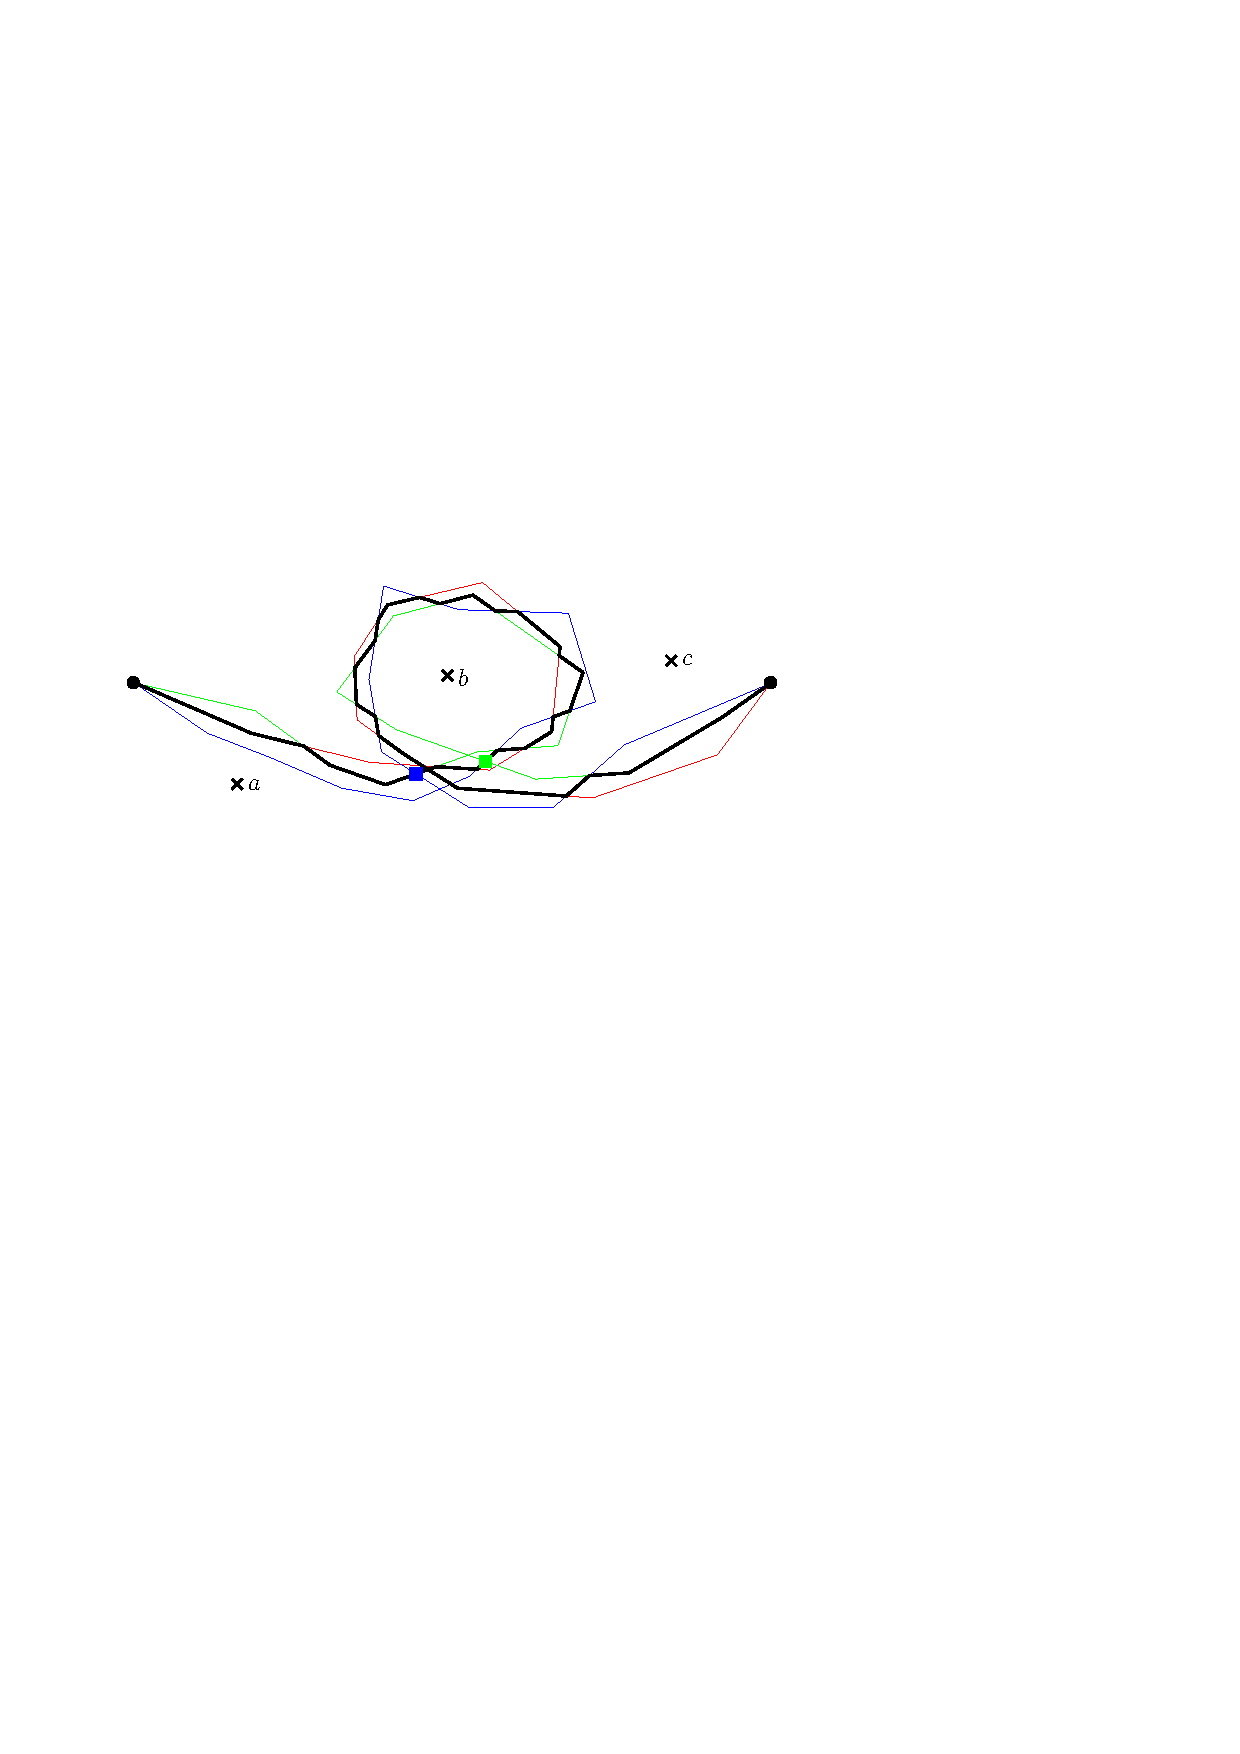
\includegraphics[scale=1]{Gambar/hmtp_works}
\caption[Modified switching method \cite{Lionov:2009}]{Modified switching method \cite{Lionov:2009}} 
\label{fig:homotopy_algo}
\end{figure}

If the median switches at this intersection, the final signature will be \textit{$a^{+}b^{-}c^{-}$}, which is not the signature of this set (\textit{$a^{+}b^{-}b^{+}b^{-}c^{-}$}). 
At this point, the median does not switch to another trajectory. 
Instead, it continues to move along the green trajectory. 
The same situation also occurs when the median (now following the blue trajectory) intersects with the green trajectory (at the small green square).

Although this algorithm can produce a more suitable median trajectory for the situation where the switching method fails, the quality of the homotopic median trajectory depends heavily on the following factors:
\begin{itemize}
\item placement of the crosses
\item the number of trajectories which have the same signature 
\end{itemize}

Therefore, in several cases the algorithm with the homotopy concept cannot produce suitable median trajectories.
We give two examples in Figure~\ref{fig:homotopy_fail0}: in the left-hand side of figure, the final median trajectory (blue) does not follow other trajectories to the area with a narrow space. 
This problem arises because that narrow space is not large enough for a cross to be placed. 

\begin{figure}
\centering
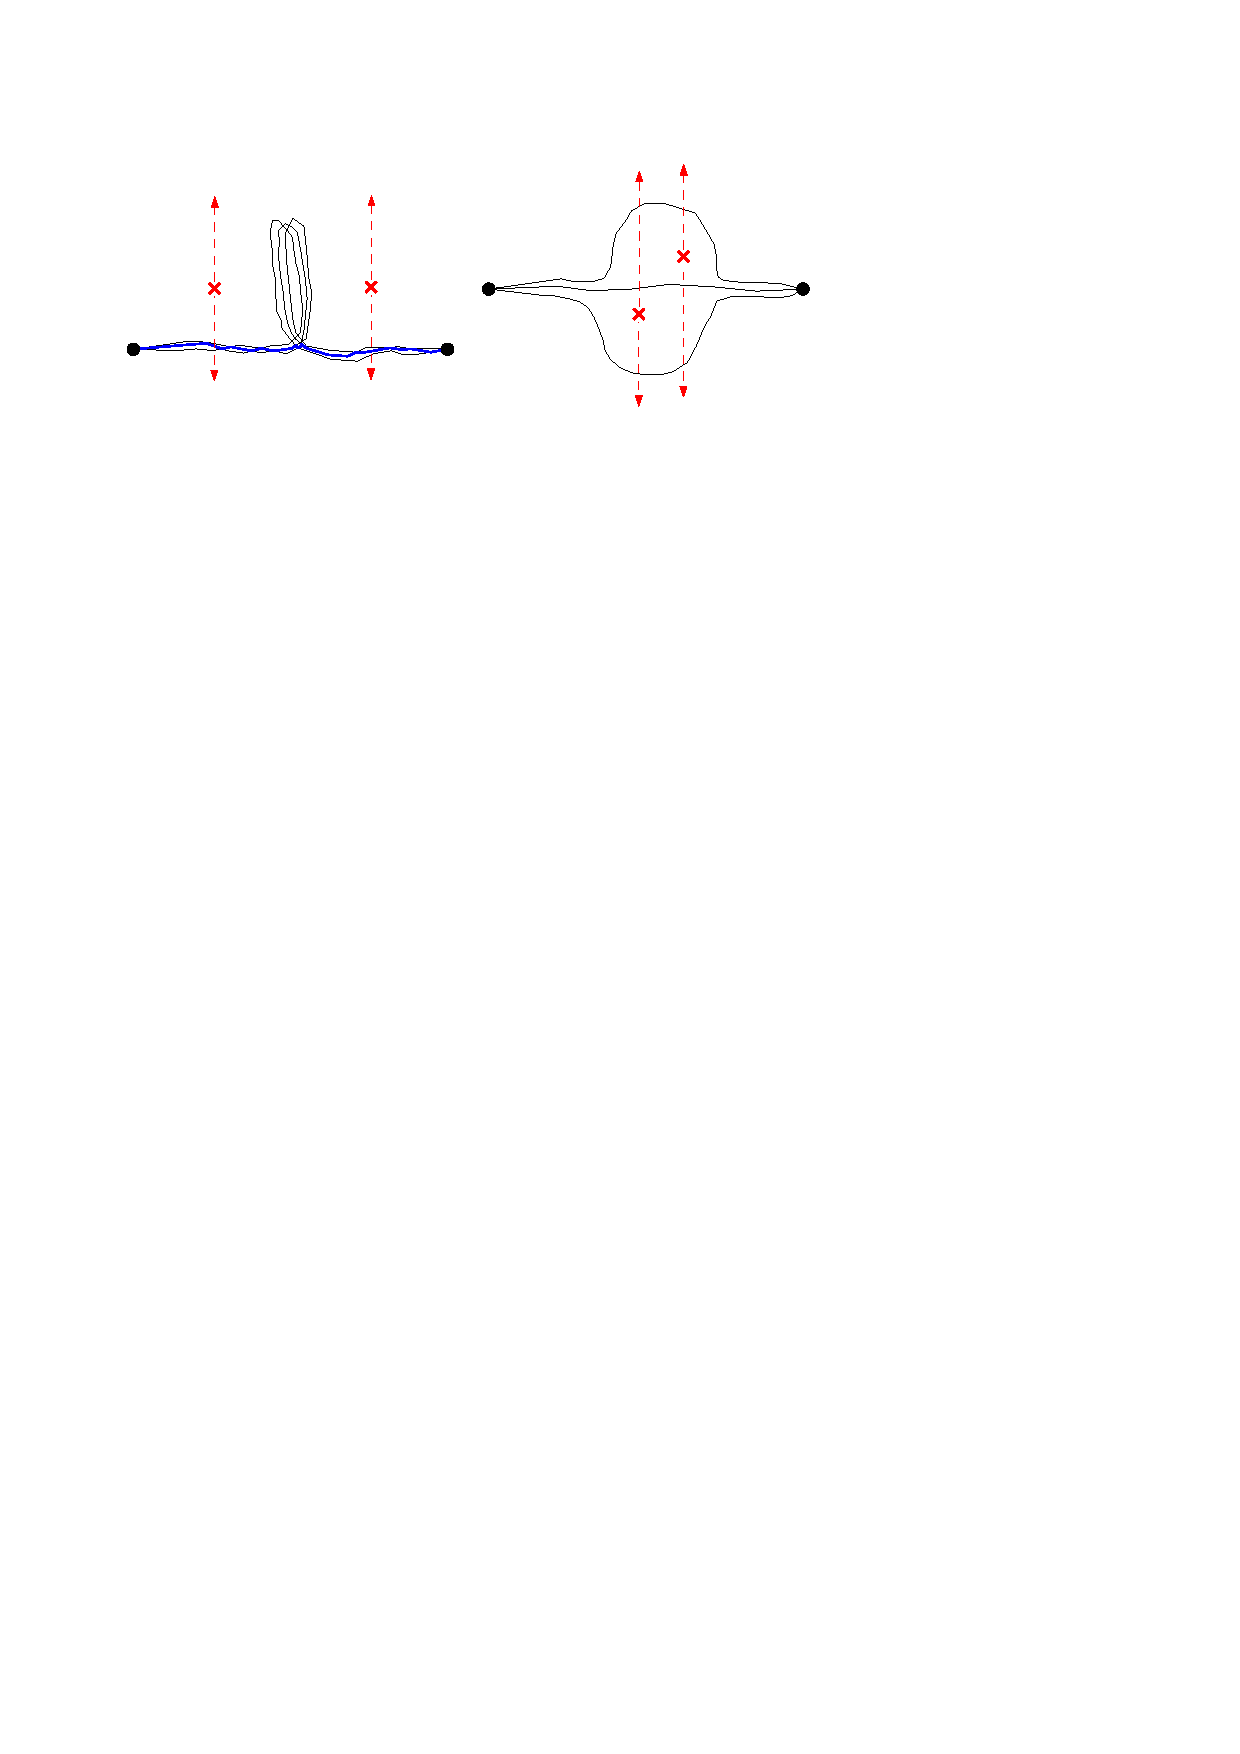
\includegraphics[scale=1]{Gambar/homotopy_fail0}
\caption[Example cases where algorithm using homotopy will fail]{Example cases where algorithm using homotopy will fail} 
\label{fig:homotopy_fail0}
\end{figure}

In the right-hand side of the figure, there are no two trajectories homotopically equivalent to each other. 
Nevertheless, by looking at their position, the median trajectory should be the one in the middle (between the two crosses).
However, the algorithm with the homotopy concept does not guarantee that a suitable median trajectory will be found because there is no subset that contains the majority of trajectories in $T$. 
Figure~\ref{fig:homotopy_fail1} shows an example from \cite{Lionov:2009}, where the median trajectory does not completely follow what other trajectories do.

\begin{figure}
\centering
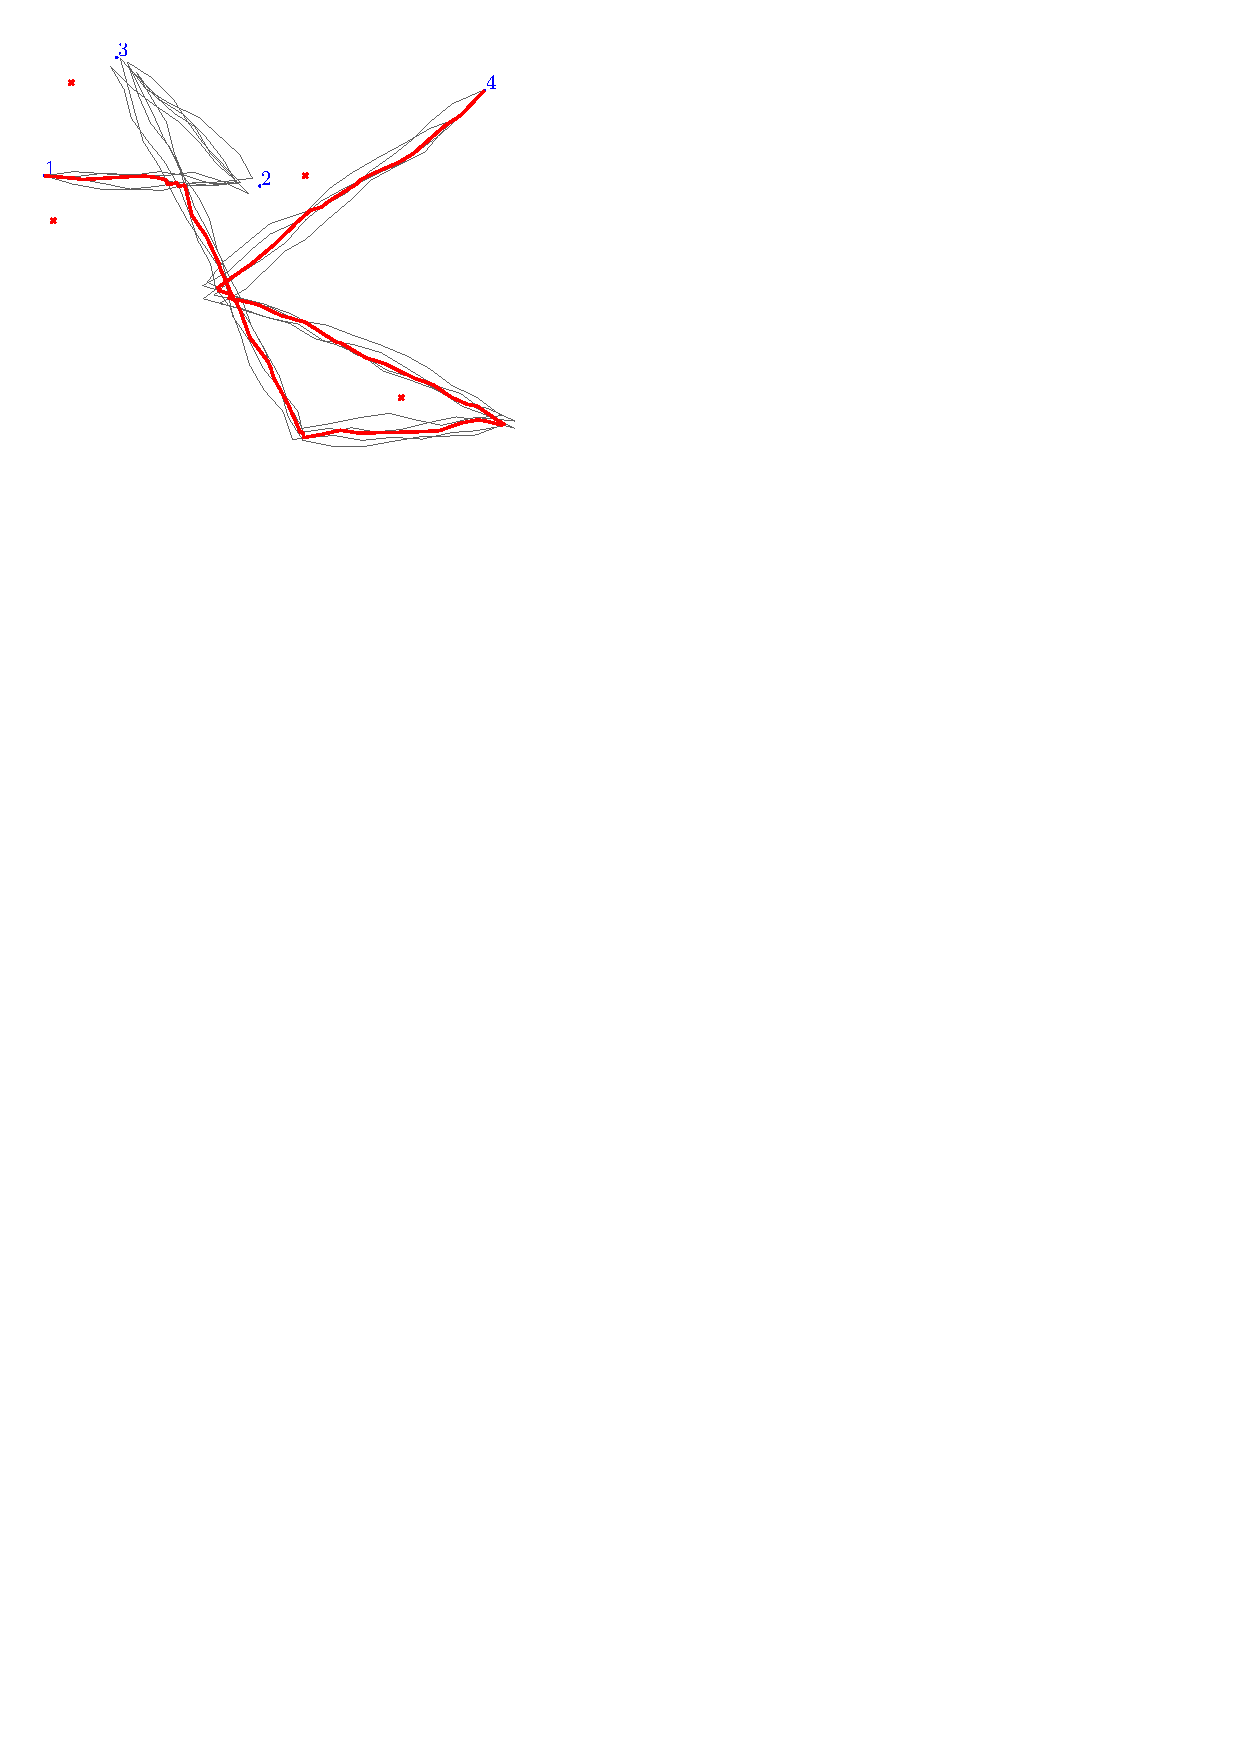
\includegraphics[scale=1]{Gambar/homotopy_fail1}
% \caption[The median trajectory does not pass through part of trajectories in the upper left area]{The median trajectory does not pass through part of trajectories in the upper left area} 
\caption{The median trajectory does not pass through part of trajectories in the upper left area}
\label{fig:homotopy_fail1}
\end{figure}

\subsection{The Proposed Solutions}
\label{sec:solution}

To solve the problems we mention in the previous section, we propose two algorithms to compute the median trajectory from a set of $m$ trajectories (where each trajectory has $n$ segments).

The first algorithm is an $O(1.2108^{m} + m^{5}n^{5})$ worst-case time algorithm.
This algorithm uses the Fr\'{e}chet Distance \cite{AltGodau:1995} and works similar to the algorithm using the homotopy concept because both of them have to create the largest subset of similar trajectories and then compute the median trajectory by using parts of trajectories in that subset. 
By using the Fr\'{e}chet Distance, we avoid the requirement to find proper places to put crosses, but still can produce suitable median trajectory in the situation where the homotopic algorithm fails (e.g. the example with a narrow space).

The second algorithm uses the combination of the buffer concept and Dijkstra's Shortest Path algorithm.
Unlike all previous algorithms, this algorithm does not need to find the largest subset consisting similar trajectories. 
% Thus, it will solve the second problem from the homotopy concept, where each trajectory is different from each other .
Using this algorithm, we can compute the median trajectory in $O(h^{2} \log h)$ time in the worst-case, where $h$ is the number of all segments in $T$ $(h = O(mn))$.

We implemented the second algorithm in Java programming language and experiments have been done to determine the quality of the resulting median trajectory produced by this algorithm.
To provide the test data (set of trajectories), we use a trajectories generator instead of using real-world data.
This allow us to test much larger sets of trajectories

\section{Outline of the Thesis}
\label{sec:outline}

Chapter \ref{chap:definition} describes the properties for a set of trajectories and also some properties the median trajectory should have.

The next two chapters explain in detail the two algorithms:
\begin{itemize}
\item 
Chapter 3 starts with a brief introduction of the Fr\'{e}chet Distance and after that, we will explain how to use it to compute the median trajectory. 
\item 
Chapter 4 introduces the method to compute the median trajectory using the combination of the buffer concept and Dijkstra's shortest path algorithm. 
\end{itemize}

We will give an explanation about our implementation, particularly on the implementation of the trajectories generator, in Chapter 5.
In Chapter 6, we present the measures used to evaluate the quality of the median trajectory, the experiments set-up and the results from the experiments.
This thesis will be concluded in Chapter 7 and 8, where we draw conclusions and discuss some issues and possible directions for further research.

\lipsum[1-14]